\documentclass[11pt,a4paper]{article}

% ------------------------------------------------------------------
% Packages
% ------------------------------------------------------------------
\usepackage[T1]{fontenc}
\usepackage[utf8]{inputenc}
\usepackage{lmodern}
\usepackage{microtype}
\usepackage[a4paper,margin=2.5cm,headheight=14pt]{geometry}
\usepackage{amsmath,amssymb,amsthm,mathtools,bm}
\usepackage{graphicx}
\usepackage{booktabs,tabularx,multirow,longtable}
\usepackage{float}
\usepackage{xcolor}
\usepackage{enumitem}
\usepackage{fancyhdr}
\usepackage{caption}
\usepackage{subcaption}
\usepackage{algorithm}
\usepackage{algpseudocode}
\usepackage{tikz}
\usetikzlibrary{arrows.meta,positioning,shapes.geometric,fit,calc,backgrounds}
\usepackage{tcolorbox}
\tcbuselibrary{skins,breakable}
\usepackage[round,authoryear]{natbib}
\usepackage[hidelinks]{hyperref}
\newcommand{\cref}[1]{\autoref{#1}}
\newcommand{\Cref}[1]{\autoref{#1}}
\renewcommand{\sectionautorefname}{Section}
\renewcommand{\subsectionautorefname}{Section}
\renewcommand{\subsubsectionautorefname}{Section}
\renewcommand{\equationautorefname}{Equation}
\renewcommand{\figureautorefname}{Figure}
\renewcommand{\tableautorefname}{Table}
\newcommand{\algorithmautorefname}{Algorithm}
\newcommand{\propositionautorefname}{Proposition}

\graphicspath{{../outputs/figures/}}

% ------------------------------------------------------------------
% Style
% ------------------------------------------------------------------
\definecolor{accent}{HTML}{1F4E79}
\definecolor{soft}{HTML}{EAF1F8}
\definecolor{warnsoft}{HTML}{FFF4E5}
\definecolor{warnline}{HTML}{C77700}

\hypersetup{colorlinks=true,linkcolor=accent,citecolor=accent,urlcolor=accent}
\captionsetup{font=small,labelfont=bf}
\setlist{itemsep=2pt,topsep=4pt}
\renewcommand{\arraystretch}{1.15}

\pagestyle{fancy}
\fancyhf{}
\fancyhead[L]{\small\textcolor{accent}{Temporal Semantic Hypergraph Coarsening}}
\fancyhead[R]{\small\nouppercase{\leftmark}}
\fancyfoot[C]{\small\thepage}
\renewcommand{\headrulewidth}{0.4pt}

\newtheorem{definition}{Definition}[section]
\newtheorem{proposition}{Proposition}[section]
\theoremstyle{remark}
\newtheorem{remark}{Remark}[section]

\newtcolorbox{keybox}[1][]{colback=soft,colframe=accent,boxrule=0.6pt,arc=2pt,
  left=6pt,right=6pt,top=4pt,bottom=4pt,fonttitle=\bfseries\small,title={#1}}
\newtcolorbox{cautionbox}[1][]{colback=warnsoft,colframe=warnline,boxrule=0.6pt,arc=2pt,
  left=6pt,right=6pt,top=4pt,bottom=4pt,fonttitle=\bfseries\small,title={#1}}

\newcommand{\code}[1]{\texttt{\small #1}}
\newcommand{\VI}{\operatorname{VI}}
\newcommand{\ARI}{\operatorname{ARI}}
\newcommand{\R}{\mathbb{R}}
\DeclareMathOperator*{\argmin}{arg\,min}
\DeclareMathOperator*{\argmax}{arg\,max}

\algrenewcommand\algorithmicrequire{\textbf{Input:}}
\algrenewcommand\algorithmicensure{\textbf{Output:}}

% ------------------------------------------------------------------
\begin{document}
% ------------------------------------------------------------------

\begin{titlepage}
\centering
\vspace*{2.5cm}
{\color{accent}\rule{\linewidth}{1.2pt}}\\[0.8cm]
{\Huge\bfseries Temporal Semantic Hypergraph Coarsening\par}
\vspace{0.5cm}
{\Large Multi-Resolution Semantic Abstraction over an\\ Evolving Knowledge Hypergraph\par}
\vspace{0.6cm}
{\color{accent}\rule{\linewidth}{1.2pt}}\\[1.6cm]
{\large\textsc{Technical Research Report}\par}
\vspace{2.2cm}
{\Large Luka Burduli\par}
\vspace{0.4cm}
{\large September 2026\par}
\vfill
\begin{minipage}{0.82\linewidth}
\small\centering
Full report accompanying the submission package \code{clean\_tshc}.
It explains the theory behind the method, how the implementation works,
how the evaluation was designed to be trustworthy, and what the results show,
including negative results.
\end{minipage}
\vspace{1.5cm}
\end{titlepage}

% ------------------------------------------------------------------
\begin{abstract}
\noindent
Scientific knowledge graphs quickly become too large to read or to search
exhaustively. This report describes \emph{Temporal Semantic Hypergraph Coarsening}
(TSHC), a method that turns an evolving knowledge \emph{hypergraph} of
materials-science and machine-learning literature (5{,}798 nodes, 1{,}429
hyperedges, 52 papers) into a nested, three-level hierarchy of super-nodes
with at most 12, 40 and 120 clusters, at four annual snapshots (2020, 2022,
2024, 2026).

The hierarchy is built bottom-up by greedy agglomerative merging that minimises a
single explicit objective. The objective combines three normalised terms:
semantic dispersion of sentence embeddings (a Ward-type term), the entropy
fragmentation of the \emph{native} hyperedges (no pairwise projection), and a
variation-of-information penalty that keeps each level close to the same level of
the previous snapshot. Laminarity and the size budgets hold by construction;
coherence, stability and label faithfulness are measured empirically.
Super-node identities are tracked across snapshots by Hungarian matching and an
overlap-based event log (birth, growth, merge, split, death).

Evaluation was designed to avoid circularity. Coherence is measured with a
\emph{different} embedding model (BGE) from the one used for construction
(MiniLM) and compared against 100 type- and size-preserving null partitions.
Stability is measured both under 10\% hyperedge deletion (five seeds, $t$-intervals)
and across real snapshots. Labels are generated from one part of each cluster and
checked by an NLI model against the held-out part. Retrieval predictions are frozen
and hashed before ground truth is read.

The temporal variant raises mean cross-snapshot ARI from 0.725 (static) to 0.892
while lowering mean final-snapshot coherence only from 0.813 to 0.811. All native
variants beat their null models, but by small absolute margins (0.003--0.011
cosine). Label quality is mixed (overclaim proxy 0.32/0.31 at levels 0/1).
Coarse-to-fine retrieval reduced comparison work by 69\% at beam 3, but neither the
hierarchy nor the flat baseline recovered any complete gold method identity in the
top 10 or 25. Positive controls show that this is a ranking failure, not an evaluator
error. These negative results are reported and analysed rather than tuned away.
\end{abstract}

\clearpage
\tableofcontents
\clearpage
\listoffigures
\listoftables
\listofalgorithms
\clearpage

% ==================================================================
\section{Introduction}
\label{sec:intro}
% ==================================================================

\subsection{Motivation}

Research literature is increasingly represented as \emph{knowledge graphs}.
Papers, methods, datasets, metrics, claims and problems become nodes, and the
relations extracted from papers become edges. Such a representation lets software
agents and people reason over a field instead of reading it paper by paper.
It also grows quickly: a few thousand papers already produce tens of thousands of
nodes. Nobody can read a graph that large, and exhaustive search over all of it
gets expensive for a retrieval agent.

What is needed is a \emph{multi-resolution semantic abstraction}: a stack of
increasingly coarse views of the same graph. A reader starts from about a dozen
macro-concepts and drills down to individual methods and papers, much like zooming
in an online map. Three properties make this harder than ordinary clustering:

\begin{enumerate}
  \item \textbf{The relations are higher-order.} One extracted relation can connect
        many entities at once. For example, a comparison table links several
        methods, a dataset and a metric. These are \emph{hyperedges}, and splitting
        them into pairs discards information.
  \item \textbf{The graph evolves.} New papers arrive every year. A hierarchy that
        reshuffles completely after every update is useless for a user who has
        learned where things are.
  \item \textbf{The result must be trustworthy.} The super-nodes need names, those
        names must not claim more than the members support, and the quality
        measurements must not be circular.
\end{enumerate}

\subsection{The assessment task}

The assessment (Constructor Knowledge Labs, Knowledge Discovery project) provides a
real Temporal Knowledge Hypergraph (TKH) export of 52 papers on machine-learning
interatomic potentials and materials science, together with 18 domain questions
and ground-truth answers. It asks for six properties, which this report refers to as
P1--P6:

\begin{description}[leftmargin=1.2cm,style=nextline]
  \item[P1] \textbf{Laminar refinement}: each level must refine the one above it.
  \item[P2] \textbf{Size budget}: level $k$ has at most $N_k$ super-nodes, with
            $N_0\approx 10$--$15$. This is a hard constraint.
  \item[P3] \textbf{Semantic coherence}: members of a super-node are close in
            meaning, not only in topology.
  \item[P4] \textbf{Hyperedge fidelity}: the method must operate on the
            hypergraph itself, and the hyperedge coarsening rule must be the one
            actually applied.
  \item[P5] \textbf{Temporal stability}: the hierarchy evolves smoothly and
            super-node identities can be tracked.
  \item[P6] \textbf{Faithful labels}: labels and glosses assert nothing that the
            members (visible at the snapshot's cutoff) do not support.
\end{description}

The task explicitly warns about a methodological hazard: measuring coherence with
the same embedding that was used to build the clusters would guarantee a high
score by construction.

\subsection{Research questions}

The work addresses four questions:

\begin{enumerate}[label=\textbf{RQ\arabic*}]
  \item How can structural (hyperedge) and semantic (text) signals be combined in
        one explicit, auditable objective that produces a laminar, budgeted
        hierarchy?
  \item Does temporal regularisation measurably improve cross-snapshot stability,
        and what does it cost in coherence?
  \item Is the resulting hierarchy more coherent than chance when measured by an
        \emph{independent} signal?
  \item Does coarse-to-fine navigation through the hierarchy help a downstream
        retrieval task compared with a flat baseline?
\end{enumerate}

\subsection{Contributions}

\begin{itemize}
  \item A formal objective $J_t$ that balances semantic dispersion, native hyperedge
        fragmentation and level-specific temporal variation of information, with
        closed-form merge costs (\cref{sec:method}).
  \item A deterministic, restricted-candidate greedy optimiser that guarantees
        laminarity and budgets and keeps every original hyperedge's identity, arity and
        multiplicity at every level (\cref{sec:impl}).
  \item A temporal layer with Hungarian identity matching and an overlap-based
        event log.
  \item An evaluation protocol that avoids circularity: separate encoders, null
        models, perturbation confidence intervals, a held-out label check, and
        predictions frozen before ground truth is read (\cref{sec:setup}).
  \item A comparison of four variants (semantic-only, pairwise projection, static
        native, temporal native), reporting the negative results in full
        (Sections~\ref{sec:results} and~\ref{sec:discussion}).
\end{itemize}

\subsection{Structure of the report}

\Cref{sec:background} introduces the theory the method relies on.
\Cref{sec:data} describes the data and how it is cut into snapshots.
\Cref{sec:method} states the formal problem and derives the method.
\Cref{sec:impl} explains how the code implements it, module by module.
\Cref{sec:setup} describes the experimental protocol, \cref{sec:results} the
results and \cref{sec:discussion} their interpretation.
\Cref{sec:limitations} lists limitations and future work, and
\cref{sec:conclusion} concludes.

% ==================================================================
\section{Theoretical Background}
\label{sec:background}
% ==================================================================

This section introduces the concepts used in the rest of the report. It is written
so that a reader who knows basic linear algebra and probability can follow the
method without consulting the references.

\subsection{Graphs and hypergraphs}

A (simple, undirected) \emph{graph} $G=(V,E)$ consists of a node set $V$ and a set
of edges $E\subseteq\{\{u,v\}:u,v\in V\}$. Every edge joins exactly two nodes.

\begin{definition}[Hypergraph]
A \emph{hypergraph} $H=(V,E)$ has a node set $V$ and a collection $E$ of
\emph{hyperedges}, where each hyperedge $e\in E$ is a subset $e\subseteq V$ with
$|e|\ge 2$. The \emph{arity} (or size) of $e$ is $r_e=|e|$. Hyperedges carry
attributes such as a relation type, a year and a provenance record.
\end{definition}

An ordinary graph is a hypergraph in which every arity equals~2. Hypergraphs
represent many-to-many relations directly. In the knowledge hypergraph used here, a
single \code{evaluated\_on} relation can connect a method, several datasets and
several metrics at the same time.

\paragraph{Clique projection.}
The most common way to reuse graph algorithms on a hypergraph is the \emph{clique
expansion}: every hyperedge of arity $r$ is replaced by all $\binom{r}{2}$ node
pairs, often weighted by $1/\binom{r}{2}$ so that each hyperedge contributes a total
weight of one. The projection is lossy, as \cref{fig:projection} shows.

\begin{figure}[!htbp]
\centering
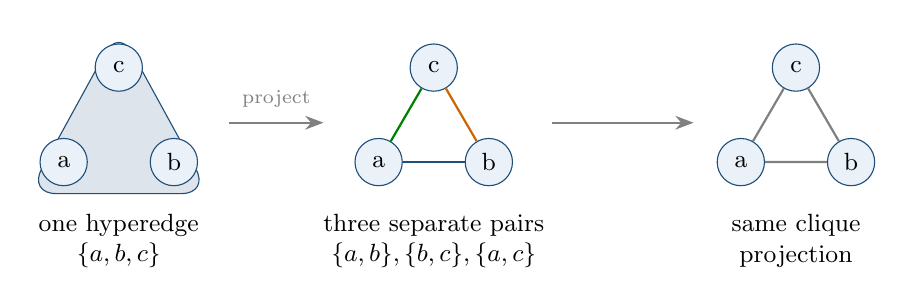
\begin{tikzpicture}[
  node distance=1.1cm,
  v/.style={circle,draw=accent,fill=soft,minimum size=6mm,inner sep=0pt,font=\small}]
  % left: two hyperedges
  \begin{scope}
    \node[v] (a) at (0,0) {a};
    \node[v] (b) at (1.4,0) {b};
    \node[v] (c) at (0.7,1.2) {c};
    \begin{scope}[on background layer]
      \draw[fill=accent!15,draw=accent,rounded corners=10pt]
        (-0.45,-0.4) -- (1.85,-0.4) -- (0.7,1.7) -- cycle;
    \end{scope}
    \node[font=\small,align=center] at (0.7,-1.0) {one hyperedge\\$\{a,b,c\}$};
  \end{scope}
  \begin{scope}[xshift=4.0cm]
    \node[v] (a2) at (0,0) {a};
    \node[v] (b2) at (1.4,0) {b};
    \node[v] (c2) at (0.7,1.2) {c};
    \draw[thick,accent] (a2)--(b2);
    \draw[thick,orange!80!black] (b2)--(c2);
    \draw[thick,green!50!black] (a2)--(c2);
    \node[font=\small,align=center] at (0.7,-1.0) {three separate pairs\\$\{a,b\},\{b,c\},\{a,c\}$};
  \end{scope}
  \begin{scope}[xshift=8.6cm]
    \node[v] (a3) at (0,0) {a};
    \node[v] (b3) at (1.4,0) {b};
    \node[v] (c3) at (0.7,1.2) {c};
    \draw[thick,gray] (a3)--(b3) (b3)--(c3) (a3)--(c3);
    \node[font=\small,align=center] at (0.7,-1.0) {same clique\\projection};
  \end{scope}
  \draw[-{Stealth},thick,gray] (2.1,0.5) -- (3.3,0.5);
  \draw[-{Stealth},thick,gray] (6.2,0.5) -- (8.0,0.5);
  \node[font=\scriptsize,gray] at (2.7,0.8) {project};
\end{tikzpicture}
\caption{Why clique projection loses information: a single ternary hyperedge and
three independent pairwise relations produce the same projected graph (up to
weights). The projection cannot say which situation it came from.}
\label{fig:projection}
\end{figure}

A projected graph cannot distinguish ``$a$, $b$ and $c$ were stated together in one
relation'' from ``three unrelated papers each related two of them''. Once pair
weights from overlapping hyperedges are summed, the source hyperedges, their arities
and their groupings can no longer be recovered. \Cref{sec:data} quantifies this loss
on the actual data.

\subsection{Partitions, hierarchies and laminarity}

\begin{definition}[Partition]
A \emph{partition} $P=\{C_1,\dots,C_K\}$ of $V$ is a set of non-empty, pairwise
disjoint \emph{clusters} whose union is $V$. We write $P(v)$ for the cluster that
contains $v$.
\end{definition}

\begin{definition}[Refinement and laminar hierarchy]
A partition $P'$ \emph{refines} $P$ (written $P'\preceq P$) if every cluster of $P'$
is contained in exactly one cluster of $P$. A sequence
$P_K\preceq P_{K-1}\preceq\dots\preceq P_0$ is a \emph{laminar} (nested) hierarchy:
any two clusters from any levels are either disjoint or one contains the other.
Each cluster at level $k+1$ has a unique parent at level $k$.
\end{definition}

A hierarchy can be drawn as a tree (a \emph{dendrogram}), with the whole node set at
the root, the coarsest clusters below it, and individual nodes as leaves.

\subsection{Agglomerative clustering and Ward's criterion}

\emph{Agglomerative} (bottom-up) hierarchical clustering starts from singletons and
repeatedly merges the two clusters whose merge is cheapest under some criterion. It
has two properties that matter here:

\begin{enumerate}
  \item Merging only ever unites clusters, so if we record the partition at chosen
        numbers of clusters (e.g.\ 120, then 40, then 12), the recorded partitions
        are automatically nested. \textbf{Laminarity is free.}
  \item The number of clusters falls by exactly one per merge, so stopping at any
        budget $N$ is trivial. \textbf{Budgets are free.}
\end{enumerate}

\paragraph{Ward's criterion.}
Let $x_v\in\R^d$ be the feature vector of node $v$. For a cluster $C$ with centroid
$\mu_C=\frac1{|C|}\sum_{v\in C}x_v$, the within-cluster sum of squares is
$\mathrm{SS}(C)=\sum_{v\in C}\|x_v-\mu_C\|^2$. \citet{ward1963} merges the pair that
increases the total within-cluster sum of squares the least. The increase has a
closed form:
\begin{equation}
  \mathrm{SS}(A\cup B)-\mathrm{SS}(A)-\mathrm{SS}(B)
  \;=\;\frac{|A|\,|B|}{|A|+|B|}\,\|\mu_A-\mu_B\|^2 .
  \label{eq:ward}
\end{equation}
Only the cluster sizes and the \emph{sum} of the member vectors are needed, so each
candidate merge costs $O(d)$ to evaluate. TSHC uses \cref{eq:ward} as its semantic
term.

\paragraph{Graph coarsening.}
In scientific computing and graph learning, \emph{coarsening} means building a
smaller graph whose nodes are aggregates of the original nodes, recursively, to obtain
a multilevel representation \citep{chen2022coarsening}. Coarsening literature
stresses that one must state exactly \emph{what} a coarse representation preserves.
TSHC takes this idea literally: every original hyperedge is kept, with its identity,
arity and endpoint multiplicities, at every level (\cref{sec:collapse}).

\paragraph{Displayed versus natural hierarchy.}
\citet{schaub2023hierarchical} point out that an algorithm can always produce a
hierarchy, but that this is different from showing that the data \emph{has}
identifiable hierarchical community structure. TSHC produces a hierarchy with fixed
\emph{display budgets} and makes no claim that 12/40/120 are natural community
counts.

\subsection{Entropy and hypergraph clustering}

For a discrete distribution $p=(p_1,\dots,p_K)$ the Shannon entropy is
$H(p)=-\sum_i p_i\log p_i$, with $0\log 0=0$. It is zero for a point mass and at most
$\log K$, the value for a uniform distribution.

Consider a hyperedge $e$ of arity $r_e$ and a partition $P$. The fraction of the
edge's endpoints in cluster $C$ is $p_{e,C}=|e\cap C|/r_e$. The entropy
$H_e(P)=-\sum_C p_{e,C}\log p_{e,C}$ measures how \emph{fragmented} the hyperedge is
by the partition. It is $0$ when the whole edge lies in one cluster, and it reaches
$\log r_e$ when every endpoint is in a different cluster. Dividing by $\log r_e$
gives a normalised fragmentation in $[0,1]$ that is comparable across arities.

\citet{zhou2006hypergraph} established that hypergraph clustering should treat
multi-node relations as units instead of immediately reducing them to pairs. They did
this with a normalised spectral hypergraph cut. TSHC keeps the principle (penalise
cutting a hyperedge, with the edge as the unit) but uses entropy fragmentation, which
has an exact, cheap merge update (\cref{sec:deltas}).

\subsection{Comparing partitions: ARI and variation of information}
\label{sec:bg-compare}

Stability evaluation and the temporal regulariser both need a way to compare two
partitions $P$ and $Q$ of the same $n$ elements.

\paragraph{Contingency table.}
Let $n_{ij}=|P_i\cap Q_j|$, with row sums $a_i=|P_i|$ and column sums $b_j=|Q_j|$.

\paragraph{Adjusted Rand Index.}
The Rand index counts the fraction of element pairs on which the two partitions
agree (both together or both apart). \citet{hubert1985} corrected it for chance:
\begin{equation}
\ARI(P,Q)=\frac{\sum_{ij}\binom{n_{ij}}{2}-\Big[\sum_i\binom{a_i}{2}\sum_j\binom{b_j}{2}\Big]\Big/\binom{n}{2}}
{\tfrac12\Big[\sum_i\binom{a_i}{2}+\sum_j\binom{b_j}{2}\Big]-\Big[\sum_i\binom{a_i}{2}\sum_j\binom{b_j}{2}\Big]\Big/\binom{n}{2}} .
\end{equation}
ARI equals $1$ for identical partitions and has expectation $0$ for random
partitions with the same cluster sizes. It can be negative. Because it is based on
pairs, large clusters dominate it.

\paragraph{Variation of information.}
With joint entropy $H(P,Q)=-\sum_{ij}\frac{n_{ij}}{n}\log\frac{n_{ij}}{n}$, the
variation of information \citep{meila2007} is
\begin{equation}
  \VI(P,Q)=H(P\mid Q)+H(Q\mid P)=2H(P,Q)-H(P)-H(Q).
  \label{eq:vi}
\end{equation}
VI is a true metric on partitions. It is $0$ exactly when $P=Q$ and is bounded above
by $\log n$ and, for at most $K$ clusters, by $2\log K$. It is information-theoretic
rather than pair-based, so it responds differently from ARI to changes in small
clusters. The normalised form $\VI/(2\log n)$ is used below. A useful property for
optimisation is that $\VI$ depends only on sums of $x\log x$ terms over the contingency
table, so merging two clusters of $P$ changes it by an amount that can be computed
from those two clusters' rows alone.

\subsection{Evolutionary clustering}

\emph{Evolutionary clustering} handles data that arrive over time.
\citet{chi2007evolutionary} formulate it as a trade-off between a
\emph{snapshot cost} (how well the clustering fits current data) and a
\emph{temporal cost} (how far it moves from the previous clustering):
\[
  \text{cost}_t \;=\; \text{snapshot cost}(P_t)\;+\;\lambda\cdot\text{temporal cost}(P_t,P_{t-1}).
\]
A larger $\lambda$ gives smoother but potentially less accurate clusterings. TSHC
adopts this structure, using VI on shared nodes as the temporal cost at every
hierarchy level.

\subsection{The assignment problem and the Hungarian algorithm}

Even a stable clustering needs \emph{identities}: we want to say that super-node
``L0\_2020\_0007'' in 2024 is the same concept as in 2022. Given an $m\times n$
similarity matrix $S$ between old and new clusters, we seek a one-to-one matching
$\sigma$ maximising $\sum_i S_{i,\sigma(i)}$. This is the linear assignment problem.
The Hungarian algorithm \citep{kuhn1955} solves it exactly in $O(K^3)$. As the
similarity, TSHC uses the Jaccard index
$J(A,B)=|A\cap B|/|A\cup B|$ between member sets.

\subsection{Text representations}

\paragraph{Sentence embeddings.}
Sentence-BERT \citep{reimers2019sbert} fine-tunes a transformer encoder so that the
mean-pooled output of a sentence is a vector whose cosine similarity reflects semantic
similarity. With unit-normalised vectors, cosine similarity equals the dot product and
$\|x-y\|^2=2-2\cos(x,y)\in[0,4]$. Two different families are used here:
\begin{itemize}
  \item \textbf{all-MiniLM-L6-v2} \citep{wang2020minilm}: a 6-layer distilled model
        with 384-dimensional output, used \emph{only for constructing} the hierarchy
        and labels.
  \item \textbf{BGE-small-en-v1.5} \citep{xiao2023bge}: a separately trained
        retrieval-oriented embedding model, also 384-dimensional, used
        \emph{only for evaluation} (coherence) and for the retrieval task.
\end{itemize}

\paragraph{TF-IDF.}
Term frequency--inverse document frequency weights an $n$-gram $w$ in text $d$ by
$\mathrm{tf}(w,d)\cdot\big(\log\frac{1+N}{1+\mathrm{df}(w)}+1\big)$, where $N$ is the
number of texts and $\mathrm{df}(w)$ the number containing $w$ (the smoothed
scikit-learn form), followed by $\ell_2$ normalisation. Terms that are frequent in a document but
rare overall get high weight \citep{salton1988}. TSHC uses TF-IDF over 1--3-grams to choose a cluster's
label phrase.

\subsection{Natural language inference}

Natural language inference (NLI) is the task of deciding whether a \emph{premise}
text entails, contradicts, or is neutral towards a \emph{hypothesis}. Cross-encoders
such as DeBERTa-v3 \citep{he2021debertav3}, trained on SNLI and MultiNLI-style data
\citep{bowman2015snli,williams2018mnli},
output a probability distribution over the three classes. TSHC uses NLI as an
automatic \emph{faithfulness proxy}: the premise is evidence the labeller never saw,
the hypothesis is the generated gloss, and a gloss that is not entailed counts as a
potential overclaim. The proxy is imperfect because general-domain NLI models are not
trained on materials science, and vague statements are easy to entail.

\subsection{Dense retrieval and hierarchical beam search}

In \emph{dense retrieval}, queries and documents are embedded in the same vector
space and documents are ranked by cosine similarity. A \emph{flat} retriever compares
the query with every document, which costs $n$ comparisons. A \emph{hierarchical}
retriever represents each cluster by the centroid of its documents, keeps the $b$ best
clusters at the top level (the \emph{beam}), expands only their children, and so on
down to the leaves. With a balanced hierarchy the work drops sharply. The risk is that
a relevant document inside a cluster whose centroid does not look relevant is pruned
early. The size of the beam trades recall against work.

\subsection{Statistical tools}

\paragraph{Null models and permutation tests.}
A raw coherence of 0.82 means nothing without a reference, because embedding models
make \emph{all} texts in one domain fairly similar. A \emph{null model} creates random
partitions that share every property except the one being tested. The observed value
is compared with the null distribution. With $R$ null replicates, the one-sided
empirical $p$-value is
\begin{equation}
  p=\frac{1+\#\{r:\ \text{null}_r\ge\text{observed}\}}{R+1},
\end{equation}
which is never zero. Its smallest possible value is $1/(R+1)$, which is
$1/101\approx0.0099$ for $R=100$.

\paragraph{Effect sizes.}
The absolute effect is the observed value minus the null mean. The standardised effect
divides it by the null standard deviation. A large standardised effect can arise
from a tiny absolute difference when the null distribution is very narrow, so both are
reported.

\paragraph{Confidence intervals from few seeds.}
For $n$ repeated measurements with mean $\bar x$ and sample standard deviation $s$,
the Student-$t$ 95\% interval is $\bar x\pm t_{0.975,n-1}\,s/\sqrt n$. With $n=5$,
$t_{0.975,4}\approx2.776$, so intervals are wide. They describe variation across
deletion seeds, not across corpora.

% ==================================================================
\section{Data and Temporal Snapshots}
\label{sec:data}
% ==================================================================

\subsection{The supplied knowledge hypergraph}

The input is the supplied TKH export \code{tkh\_collection10.json}. It covers 52
papers on machine-learning interatomic potentials and computational materials
science. Before any clustering, a data audit (\code{scripts/audit\_data.py})
recomputes the SHA-256 hash and schema of every input file and verifies the key
counts. Nothing in the original inputs is modified.

\begin{table}[!htbp]
\centering
\caption{Verified input audit. The benchmark contains 18 questions, not 17 as the
supplied README states.}
\label{tab:audit}
\begin{tabular}{lr@{\hspace{1.5cm}}lr}
\toprule
Item & Count & Item & Count\\
\midrule
Nodes & 5{,}798 & Article nodes & 52\\
Hyperedges & 1{,}429 & Author nodes & 318\\
Node types & 12 & Questions (Type A / Type B) & 18 (14 / 4)\\
Relation types & 11 & Gold target occurrences & 63\\
Arity range & 2--65 & Expected claims (A / B) & 224 (188 / 36)\\
\bottomrule
\end{tabular}
\end{table}

Every node has an \code{id}, a \code{type}, a \code{surface\_form} (its text), four
date fields and a \code{provenance} record. Every hyperedge has an \code{id}, a
\code{relation\_type}, a list of \code{members}, a \code{year} and a
\code{provenance} record. \Cref{tab:types} shows the composition.

\begin{table}[!htbp]
\centering
\caption{Node types and relation types in the full graph (2026 snapshot).}
\label{tab:types}
\begin{minipage}[t]{0.45\linewidth}\centering
\begin{tabular}{lr}
\toprule
Node type & Count\\
\midrule
technique & 962\\
component & 855\\
task & 732\\
claim & 690\\
problem & 634\\
cited\_work & 580\\
method & 448\\
author & 318\\
dataset & 259\\
future\_topic & 178\\
metric & 90\\
article & 52\\
\bottomrule
\end{tabular}
\end{minipage}\hfill
\begin{minipage}[t]{0.5\linewidth}\centering
\begin{tabular}{lr}
\toprule
Relation type & Count\\
\midrule
claims & 690\\
evaluated\_on & 301\\
presents & 52\\
addresses & 51\\
solves & 51\\
uses\_technique & 51\\
authored\_by & 51\\
uses\_component & 50\\
extends & 50\\
proposes\_future\_work & 45\\
cites & 37\\
\bottomrule
\end{tabular}
\end{minipage}
\end{table}

\subsection{Strict temporal visibility}
\label{sec:visibility}

The graph is not pre-cut into snapshots, so defining ``what is known at year $t$'' is
itself a modelling decision. The metadata distinguishes \code{origin\_year} (when an
entity was introduced in the world) from \code{first\_seen\_year} (the earliest
corpus paper mentioning it). For temporal honesty (P6), a snapshot may contain only
what the \emph{corpus} had seen by year $t$. TSHC therefore uses a strict visibility
rule:

\begin{definition}[Visibility]
A node $v$ is visible at $t$ iff $\mathrm{first\_seen\_year}(v)\le t$. A hyperedge
$e$ is visible at $t$ iff (i) $\mathrm{year}(e)\le t$, (ii) the year of the article
that asserts it is $\le t$ when known, and (iii) every endpoint of $e$ is visible at
$t$. The snapshot is $H_t=(V_t,E_t)$ with all visible nodes and hyperedges.
\end{definition}

Condition (iii) matters because the data contain inconsistencies. The audit function
\code{snapshots.anomalies} found:
\begin{itemize}
  \item \textbf{170} hyperedges whose \code{year} precedes the first-seen year of at
        least one endpoint, and
  \item \textbf{134} hyperedges whose \code{year} precedes the publication year of the
        article asserting them.
\end{itemize}
For example, hyperedges \code{h\_00351}--\code{h\_00355} have \code{year}~2021, but
their endpoints only become visible in 2024. Instead of silently including dangling
edges, the whole edge is deferred until all its requirements are met. As a result,
strict snapshot edge counts are below the task guide's illustrative counts
($\approx$405/589/1063 for 2020/2022/2024), which used the edge \code{year} alone.

\begin{cautionbox}[Limitation: annual resolution]
Dates are annual. The benchmark questions ask what was known ``by February 2026'', but
the 2026 snapshot contains all 2026 material, so the implementation \emph{cannot
guarantee} exclusion of material appearing after February 2026. Surface forms and
pretrained language models are also not historically versioned.
\end{cautionbox}

\subsection{Snapshot statistics}

Four snapshots are used: 2020, 2022, 2024 and 2026 (cumulative).

\begin{table}[!htbp]
\centering
\caption{Strict annual snapshots. Growth is relative to the previous snapshot.
``Deferred'' counts anomalous edges whose own year is $\le t$ but which are held back
because an endpoint or the asserting article is not yet visible.}
\label{tab:snapshots}
\small
\begin{tabular}{lrrrrrrrr}
\toprule
Year & Nodes & Edges & \multicolumn{1}{c}{Node} & \multicolumn{1}{c}{Edge} & Mean & Max & Arity & Deferred\\
 & & & \multicolumn{1}{c}{growth} & \multicolumn{1}{c}{growth} & arity & arity & ${>}2$ & \\
\midrule
2020 & 1{,}505 & 374   & ---     & ---     & 5.57 & 45 & 70.9\% & 31\\
2022 & 2{,}164 & 526   & +43.8\% & +40.6\% & 5.83 & 59 & 73.4\% & 63\\
2024 & 4{,}164 & 983   & +92.4\% & +86.9\% & 6.19 & 65 & 78.6\% & 80\\
2026 & 5{,}798 & 1{,}429 & +39.2\% & +45.4\% & 6.25 & 65 & 80.5\% & 0\\
\bottomrule
\end{tabular}
\end{table}

\begin{figure}[!htbp]
\centering
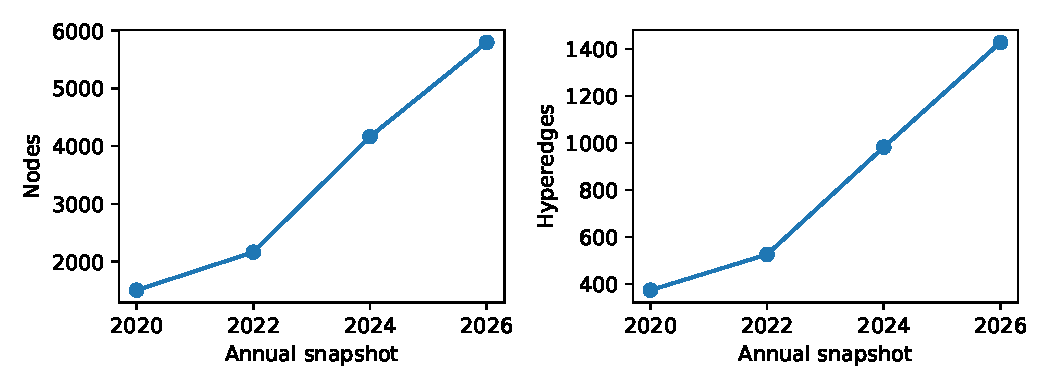
\includegraphics[width=0.85\linewidth]{snapshot_growth.pdf}
\caption{Growth of the strict annual snapshots (nodes and hyperedges).}
\label{fig:growth}
\end{figure}

The largest change is between 2022 and 2024, when the graph nearly doubles.
The snapshots are cumulative, so nodes never disappear. This later explains why no
\emph{death} events are observed.

\subsection{Arity: these are genuine hyperedges}

The median arity is 3 in every snapshot, the mean rises from 5.6 to 6.2, and by 2026
80.5\% of hyperedges have arity greater than 2 (\cref{fig:arity}). The arity
distribution is heavy-tailed, reaching 65. These relations are genuinely higher-order,
not pairs in disguise, so the hyperedge-collapse question (\cref{sec:collapse}) has
practical consequences.

\begin{figure}[!htbp]
\centering
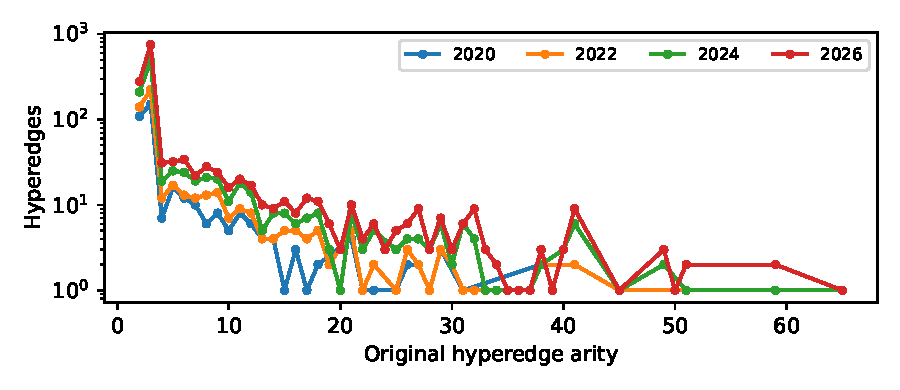
\includegraphics[width=0.85\linewidth]{arity_distribution.pdf}
\caption{Native hyperedge arity distribution across snapshots.}
\label{fig:arity}
\end{figure}

\subsection{Quantified loss of the pairwise projection}
\label{sec:projloss}

To make the cost of the clique projection concrete, the function \code{hypergraph.project}
computed it on the full graph:

\begin{itemize}
  \item 1{,}429 original hyperedges expand into \textbf{72{,}701} pair instances.
  \item These collapse into \textbf{70{,}022} unique pairs. 2{,}679 pair instances
        are repeats.
  \item \textbf{1{,}510} pairs (2.16\%) receive weight from more than one hyperedge.
        For example, the pair (\code{task\_00001}, \code{task\_00003}) is shared by
        seven different hyperedges.
\end{itemize}

After aggregation, a pair weight cannot say which hyperedges produced it, what their
arities were, or how their endpoints were grouped. The projection is the credible
simpler alternative, so it is implemented and evaluated as a baseline, but it is not the
default representation.

% ==================================================================
\section{Methodology}
\label{sec:method}
% ==================================================================

This section is the formal statement of the method (Deliverable~0 of the task). It
gives the objective, the trade-off it makes, how it is optimised, which properties
hold by construction, and its complexity.

\subsection{Problem statement}

\begin{definition}[Multi-resolution abstraction]
For each snapshot $H_t=(V_t,E_t)$, find partitions
\[
  P_3\;\preceq\;P_2\;\preceq\;P_1\;\preceq\;P_0
\]
of $V_t$, where $P_3$ consists of singletons (the leaves) and
$|P_2|\le N_2=120$, $|P_1|\le N_1=40$, $|P_0|\le N_0=12$. Every cluster at levels 0
and 1 receives a short label and a one-sentence gloss.
\end{definition}

The budgets 12/40/120 are \textbf{display budgets}, a design choice for human
navigation. They are not estimates of a natural number of communities. $N_0=12$ is
within the 10--15 range the task asks for, and each level is roughly a factor of three
finer than the one above.

\paragraph{Node representation.}
Each node $v$ is embedded as the unit vector
\[
x_v=\frac{\mathrm{MiniLM}(\text{``}\langle\text{type}\rangle\text{: }\langle\text{surface\_form}\rangle\text{''})}{\big\|\mathrm{MiniLM}(\cdot)\big\|}.
\]
Prefixing the type (e.g.\ ``dataset: OMat24'') lets the embedding tell identical
strings of different roles apart.

\subsection{The objective}

For a partition $P$ of $V_t$ with clusters $C$, centroid
$\mu_C=\frac1{|C|}\sum_{v\in C}x_v$, endpoint fractions $p_{e,C}=|e\cap C|/|e|$,
shared node set $U_t=V_t\cap V_{t-1}$ and previous partition $P_{t-1}$ at the
\emph{same level}, TSHC minimises

\begin{tcolorbox}[colback=soft,colframe=accent,boxrule=0.6pt,arc=2pt,left=2pt,right=2pt]
\begin{equation}
\begin{aligned}
J_t(P)={}&\alpha\,\underbrace{\frac{\sum_C\sum_{v\in C}\|x_v-\mu_C\|^2}{4|V_t|}}_{S(P)\text{: semantic dispersion}}
\;+\;(1-\alpha)\,\underbrace{\frac{1}{|E_t|}\sum_{e\in E_t}\frac{-\sum_C p_{e,C}\log p_{e,C}}{\log|e|}}_{F(P)\text{: hyperedge fragmentation}}\\[4pt]
&+\;\lambda\,\underbrace{\frac{\VI\!\left(P|_{U_t},\,P_{t-1}|_{U_t}\right)}{2\log|U_t|}}_{T(P,P_{t-1})\text{: temporal drift}}
\end{aligned}
\label{eq:objective}
\end{equation}
\end{tcolorbox}

\noindent with $\alpha=0.5$ and $\lambda=0.2$. $T$ is set to $0$ when fewer than two
nodes are shared, and always in the first snapshot (2020).

\paragraph{Semantic dispersion $S$.}
$S$ is the Ward within-cluster sum of squares divided by $4|V_t|$. For unit vectors,
the average squared deviation from the centroid equals $1-\|\mu_C\|^2\le1$, so
$0\le S\le 0.25$. $S$ is small when clusters contain texts with similar meaning, and it
\emph{increases} with every merge.

\paragraph{Hyperedge fragmentation $F$.}
$F$ is the average normalised entropy of each native hyperedge's endpoint distribution
across clusters, so $0\le F\le1$. At the singleton partition every hyperedge is
maximally fragmented ($F=1$), and when all nodes are in one cluster $F=0$. $F$
\emph{decreases} (or stays equal) with every merge. This term is where the hypergraph
structure enters: it rewards putting a whole relation into one super-node, and it
treats each hyperedge as a unit rather than as $\binom{r}{2}$ pairs.

\paragraph{Temporal drift $T$.}
$T$ is the variation of information between the current partition and the previous
snapshot's partition at the same level, restricted to nodes present in both, and
normalised by its upper bound $2\log|U_t|$. New nodes do not contribute: they have no
history to be faithful to.

\paragraph{The structure/semantics trade-off (P3).}
The task names reconciling structure and meaning as the central research question.
$S$ pulls towards clusters that are homogeneous in meaning regardless of relations. $F$
pulls towards clusters that contain whole relations regardless of meaning. Since $S$
only grows and $F$ only shrinks as clusters merge, the two are in genuine tension,
and $\alpha$ sets the exchange rate. $\alpha=0.5$ gives the two normalised terms equal
\emph{nominal} weight. Normalisation does not equalise their \emph{realised}
influence: $S$ is bounded by $0.25$ while $F$ ranges over $[0,1]$. The sensitivity
study (\cref{sec:sens}) shows how memberships change when $\alpha$ moves. $\lambda=0.2$
makes history a regulariser rather than a dominant force. No parameter was tuned on
the benchmark.

\subsection{Exact merge costs}
\label{sec:deltas}

Greedy agglomeration needs, for any two current clusters $A$ and $B$, the change
$\Delta J(A,B)=J(P_{A\cup B})-J(P)$. All three terms have closed forms that depend
\emph{only on the statistics of $A$ and $B$}. With $\phi(x)=x\log x$ ($\phi(0)=0$):

\paragraph{Semantic term.} From Ward's identity (\cref{eq:ward}),
\begin{equation}
\Delta S=\frac{1}{4|V_t|}\cdot\frac{n_An_B}{n_A+n_B}\,\|\mu_A-\mu_B\|^2\;\ge 0,
\end{equation}
which needs only the sizes $n_A,n_B$ and the vector sums of each cluster.

\paragraph{Fragmentation term.}
For hyperedge $e$ with arity $r$ and $m_{e,C}=|e\cap C|$ endpoints in cluster $C$,
\[
H_e=-\sum_C\frac{m_{e,C}}{r}\log\frac{m_{e,C}}{r}=\log r-\frac1r\sum_C\phi(m_{e,C}).
\]
Merging $A$ and $B$ only changes the terms for $A$ and $B$, so with edge weight $w_e$
and total weight $W$,
\begin{equation}
\Delta F=\sum_{e:\,m_{e,A}>0,\,m_{e,B}>0}\frac{w_e}{W\,r_e\log r_e}\Big[\phi(m_{e,A})+\phi(m_{e,B})-\phi(m_{e,A}+m_{e,B})\Big]\;\le 0 .
\label{eq:dF}
\end{equation}
Only hyperedges that touch \emph{both} clusters contribute, and the incidence map of the
smaller cluster suffices.

\paragraph{Temporal term.}
Let $N=|U_t|$, let $s_A$ be the number of shared nodes in $A$, and let $c_{A,k}$ be
the number of shared nodes of $A$ that were in previous cluster $k$. Writing
$H(P)=\log N-\frac1N\sum_C\phi(s_C)$ and similarly for the joint entropy, and using
\cref{eq:vi} with $H(P_{t-1})$ fixed:
\begin{align}
\Delta H(P)&=-\tfrac1N\big[\phi(s_A+s_B)-\phi(s_A)-\phi(s_B)\big],\\
\Delta H(P,P_{t-1})&=-\tfrac1N\sum_k\big[\phi(c_{A,k}+c_{B,k})-\phi(c_{A,k})-\phi(c_{B,k})\big],\\
\Delta T&=\frac{2\,\Delta H(P,P_{t-1})-\Delta H(P)}{2\log N}.
\end{align}
Only previous clusters that both $A$ and $B$ overlap contribute to the joint term.

\paragraph{Total.}
\[\Delta J(A,B)=\alpha\,\Delta S+(1-\alpha)\,\Delta F+\lambda\,\Delta T.\]
The unit test \code{test\_delta\_matches\_full\_objective} checks, on a synthetic
hypergraph and for every pair of clusters, that this incremental formula equals the
difference of the full objective recomputed from scratch, to $10^{-12}$. The test is run
both with native hyperedges and with the pairwise projection.

\subsection{Restricted-candidate greedy minimisation}

Evaluating all $\binom{n}{2}$ pairs at every step is unnecessary. Most pairs share no
meaning and no relation, so they are never good merges. TSHC restricts attention to a
\emph{candidate graph} of plausible pairs:

\begin{itemize}
  \item \textbf{Semantic proposals}: each node's 10 nearest neighbours by cosine
        similarity (the union over nodes, so the relation is symmetrised).
  \item \textbf{Structural proposals}: every pair of nodes that co-occur in some
        hyperedge (not used by the semantic-only variant).
\end{itemize}

Proposals only decide \emph{which} pairs are considered. The \emph{cost} of a pair
always uses the native objective with the original hyperedge endpoint distributions,
not the co-membership pairs. The procedure is summarised in \cref{alg:tshc}.

\begin{algorithm}[!htbp]
\caption{TSHC hierarchy construction for one snapshot}
\label{alg:tshc}
\begin{algorithmic}[1]
\Require Snapshot $H_t=(V_t,E_t)$; unit vectors $\{x_v\}$; budgets $(N_2,N_1,N_0)=(120,40,12)$; previous hierarchy $\mathcal H_{t-1}$ (optional); $\alpha,\lambda,k$
\Ensure Laminar partitions $P_3\preceq P_2\preceq P_1\preceq P_0$
\State $P\gets\{\{v\}:v\in V_t\}$; \quad $P_3\gets P$
\State $\mathcal L\gets$ kNN$_k$ pairs $\;\cup\;$ hyperedge co-membership pairs \Comment{candidate graph}
\For{$\ell = 2,1,0$}
  \State Collapse every hyperedge onto the clusters of $P$ (multiplicity counts)
  \State Load previous memberships from level $\ell$ of $\mathcal H_{t-1}$ (if any)
  \State Push $\big(\Delta J(A,B),A,B\big)$ for all $(A,B)\in\mathcal L$ into a min-heap
  \While{$|P|>N_\ell$}
    \State Pop the smallest entry whose two clusters are both still alive
    \If{heap exhausted}
       \State $(A,B)\gets$ pair with the nearest centroids \Comment{deterministic fallback}
    \EndIf
    \State $C\gets A\cup B$ \Comment{sum sizes, vector sums, incidences, history counts}
    \State $\mathrm{Nbr}(C)\gets\mathrm{Nbr}(A)\cup\mathrm{Nbr}(B)\setminus\{A,B\}$
    \For{$D\in\mathrm{Nbr}(C)$} push $\big(\Delta J(C,D),C,D\big)$ \EndFor
  \EndWhile
  \State $P_\ell\gets P$; \quad $\mathcal L\gets$ current neighbour graph (re-indexed)
\EndFor
\State \Return $(P_0,P_1,P_2,P_3)$
\end{algorithmic}
\end{algorithm}

\paragraph{Why the lazy heap is exact.}
$\Delta J(A,B)$ depends only on the sufficient statistics of $A$ and $B$ (sizes,
vector sums, incidence counts and history counts) and on global constants. It changes
only when $A$ or $B$ takes part in a merge, and then that cluster disappears and gets
a new identifier. Stale heap entries are recognisable because they mention a dead
cluster, and they are skipped. Every live candidate therefore sits in the heap with its
current cost, and each pop returns the true minimum among current candidate pairs. The
test \code{test\_heap\_matches\_exact\_current\_candidate\_minimum} verifies this.

\paragraph{The cascade.}
The three levels are built in one continuous merge sequence
$|V_t|\to120\to40\to12$. The partition is recorded when each budget is reached.
Nothing is re-clustered between levels, and the candidate graph carries over with its
union-of-neighbours updates. Between stages, the hyperedges are re-collapsed onto the
current clusters, and the temporal history is switched to the next coarser level of
the previous snapshot. For example, the $40\to12$ stage is regularised towards the
previous snapshot's level-0 partition.

\paragraph{Fallback.}
If the candidate graph ran out of pairs before the budget was reached (disconnected
components), the algorithm would deterministically merge the two clusters with the
closest centroids. In all executed runs (all variants, snapshots, perturbations and
sensitivity runs), this fallback was \textbf{never triggered}.

\begin{proposition}[Guarantees by construction]
\label{prop:laminar}
\Cref{alg:tshc} always returns partitions satisfying P1 (laminarity) and P2 (budgets).
\end{proposition}
\begin{proof}[Proof sketch]
Each step replaces two clusters by their union, so every later partition is a
coarsening of every earlier one, and each $P_\ell$ refines $P_{\ell-1}$. Each merge
lowers the number of clusters by exactly one, and the loop at level $\ell$ stops when
$|P|\le N_\ell$. The heap or the fallback always yields a pair while $|P|>1$, so the
loop terminates. The code also checks the result explicitly (\code{hierarchy.validate}):
every level covers all nodes exactly once, respects its budget, and every child cluster
has exactly one parent whose member set equals the union of its children.
\end{proof}

Greedy agglomeration makes no global optimality claim. It is a heuristic that
decreases the objective locally and deterministically.

\subsection{Hyperedge collapse (T4)}
\label{sec:collapse}

When nodes are merged into super-nodes, what happens to an arity-$n$ hyperedge whose
endpoints now fall into fewer super-nodes? TSHC maps every original hyperedge to a
\textbf{multiset of super-nodes}: a list of \code{(supernode, multiplicity)} records,
with the original identifier, relation type, provenance and arity kept.

\begin{figure}[!htbp]
\centering
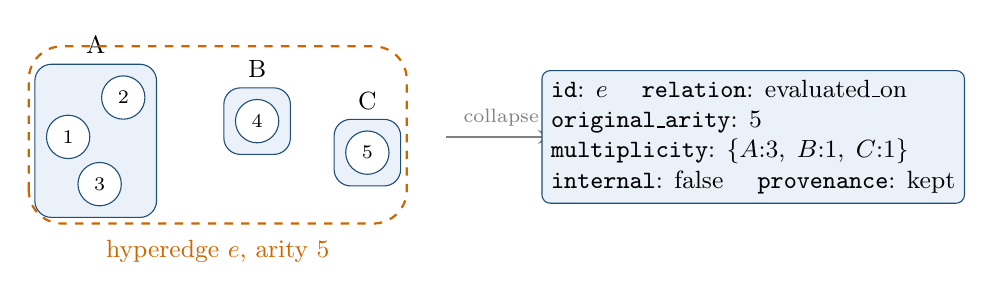
\begin{tikzpicture}[
  v/.style={circle,draw=accent,fill=white,minimum size=5.5mm,inner sep=0pt,font=\scriptsize},
  sn/.style={draw=accent,rounded corners=6pt,fill=soft}]
  % Level: fine
  \node[v] (v1) at (0,0) {1};
  \node[v] (v2) at (0.7,0.5) {2};
  \node[v] (v3) at (0.4,-0.6) {3};
  \node[v] (v4) at (2.4,0.2) {4};
  \node[v] (v5) at (3.8,-0.2) {5};
  \begin{scope}[on background layer]
    \node[sn,fit=(v1)(v2)(v3),inner sep=4pt,label=above:{\small A}] {};
    \node[sn,fit=(v4),inner sep=4pt,label=above:{\small B}] {};
    \node[sn,fit=(v5),inner sep=4pt,label=above:{\small C}] {};
  \end{scope}
  \draw[dashed,orange!80!black,thick,rounded corners=12pt]
     (-0.5,-1.1) rectangle (4.3,1.15);
  \node[font=\small,orange!80!black] at (1.9,-1.45) {hyperedge $e$, arity 5};
  % arrow
  \draw[-{Stealth},thick,gray] (4.8,0) -- (6.2,0) node[midway,above,font=\scriptsize]{collapse};
  % Record
  \node[draw=accent,fill=soft,rounded corners=3pt,align=left,font=\small] at (8.7,0)
   {\texttt{id}: $e$ \quad \texttt{relation}: evaluated\_on\\
    \texttt{original\_arity}: 5\\
    \texttt{multiplicity}: $\{A{:}3,\;B{:}1,\;C{:}1\}$\\
    \texttt{internal}: false \quad \texttt{provenance}: kept};
\end{tikzpicture}
\caption{Multiplicity-preserving collapse. Five endpoints mapping to $A,A,A,B,C$
become $\{A{:}3,B{:}1,C{:}1\}$. The multiplicities always sum to the original arity.}
\label{fig:collapse}
\end{figure}

The three cases the task asks about follow from one rule:

\begin{enumerate}
  \item \textbf{$m=n$ (all endpoints in one super-node).} The edge becomes an
        \emph{internal} hyperedge $\{A{:}n\}$, flagged \code{internal=true}. It is
        \emph{kept}, not deleted. It is evidence of why $A$ is cohesive, and the
        label packets use such internal edges.
  \item \textbf{$1<m<n$ (partly internal).} The edge becomes, for example,
        $\{A{:}m,\,B{:}n-m\}$, a coarse relation between $A$ and $B$ that remembers
        how heavily each side is involved.
  \item \textbf{$\ge3$ distinct super-nodes.} The edge remains a genuine
        higher-order relation among those super-nodes, for example
        $\{A{:}3,B{:}1,C{:}1\}$. It is never split into pairs.
\end{enumerate}

In every case $\sum_C m_{e,C}=r_e$, which the code asserts. The relation type,
provenance, identity and endpoint multiplicities remain explicit.

\paragraph{The rule is actually used.}
The collapsed records are not only an output format. At the start of each merge stage,
the hyperedges are collapsed onto the current clusters, and the multiplicities
$m_{e,C}$ \emph{are} the quantities in the fragmentation cost \cref{eq:dF}. The objective
the optimiser minimises is therefore defined on exactly the representation it outputs
(P4).

\paragraph{What the rule loses.}
From a coarse record alone one cannot say \emph{which} fine nodes inside $A$ took part.
That information needs the super-node member lists and the original input, both of
which are saved. Parallel edges with identical multisets are kept separately rather than
merged, so the coarse graph is larger than a minimal quotient would be. The rule also
does not claim that hyperedges carry information that no pairwise statistic could encode.
It only guarantees that edge identity, arity and grouping survive.

\subsection{Temporal coupling and identity tracking (T3)}

Stability comes from two separate mechanisms, and the difference matters:

\begin{enumerate}
  \item \textbf{Regularisation (causes stability).} The $\lambda T$ term makes the
        optimiser prefer merges that agree with the previous snapshot's grouping. This is
        the only mechanism that changes the clusters.
  \item \textbf{Matching (bookkeeping only).} After a hierarchy is built, super-nodes
        receive persistent identifiers by matching them with the previous snapshot's
        super-nodes. This names clusters and never changes them.
\end{enumerate}

\paragraph{Identity matching.}
At each level $\ell\in\{0,1,2\}$, compute the Jaccard similarity between every old
cluster and every new cluster, and solve the assignment problem with the Hungarian
algorithm (\code{scipy.optimize.linear\_sum\_assignment}). A new cluster matched to an
old one with non-zero overlap inherits its persistent id. Otherwise it gets a fresh id
\code{L\{level\}\_\{year\}\_\{index\}}. Leaves keep \code{leaf\_<node id>}.

\paragraph{Event log.}
From the full many-to-many overlap table (not only the matched pairs), the membership
events defined in \cref{tab:events} are recorded.

\begin{table}[!htbp]
\centering
\caption{Temporal event definitions. A \emph{strong} overlap requires at least 2 shared
nodes and at least 10\% of the relevant cluster's shared membership.}
\label{tab:events}
\begin{tabularx}{\linewidth}{lX}
\toprule
Event & Definition\\
\midrule
birth & a new cluster overlaps no old cluster\\
continuation & a new cluster inherits an id and acquired no new members\\
growth & a new cluster inherits an id and acquired at least one member\\
merge & a new cluster has strong overlaps with $\ge2$ old clusters\\
split & an old cluster has strong overlaps with $\ge2$ new clusters\\
death & an old cluster overlaps no new cluster\\
\bottomrule
\end{tabularx}
\end{table}

These events are not mutually exclusive: a cluster can both inherit an identity and
be the target of a merge. The 2-node and 10\% thresholds ignore one-node
``contamination'', which the test \code{test\_split\_merge\_ignore\_one\_node\_contamination}
checks. The events describe \emph{membership} changes. They are not claims about
scientific history.

\subsection{Label generation (T5)}
\label{sec:labels}

Labels for levels 0 and 1 are generated deterministically, without a large language
model. The central idea is a \textbf{generation/held-out split}: part of each cluster is
used to write the label, and the rest is kept back to check it. This neutralises the
circularity warned about in the task, where labeller input and faithfulness evidence
would otherwise be the same text.

\begin{enumerate}
  \item \textbf{Split.} Within each cluster and separately for each node type,
        members are ordered by $\mathrm{SHA256}(\text{seed}:\text{id})$, and the first
        $\approx70\%$ go to the \emph{generation} set, the rest to the \emph{held-out}
        set. A type with a single member goes to generation.
  \item \textbf{Phrase.} A TF-IDF model (1--3-grams, English stop words removed) is
        fitted on the surface forms of \emph{all generation members of all clusters} at
        that snapshot and level, with authors excluded. The label is the $n$-gram with
        the highest mean TF-IDF weight over the cluster's own generation members,
        ignoring $n$-grams without letters or made only of stop words, and truncated to
        6 words. Ties go to the phrase that occurs in the most central representative,
        then alphabetically. The fallback label is ``Scientific evidence''.
  \item \textbf{Representatives.} Generation members (non-author) are ranked by cosine
        similarity to the \emph{generation-only} MiniLM centroid. The top two names of
        at most 100 characters are quoted.
  \item \textbf{Gloss.} A conservative template:
        \emph{``This cluster groups evidence concerning $\langle$label$\rangle$,
        including $\langle$rep$_1\rangle$; $\langle$rep$_2\rangle$.''}
\end{enumerate}

The template deliberately claims only that the cluster \emph{contains} evidence about
the phrase, which is the weakest claim that is still informative. Temporal honesty
holds because generation uses only nodes and hyperedges visible in the snapshot, which
the code asserts. The exact generation input of every label (members, type counts,
internal hyperedges, phrase, representatives) is saved under
\code{outputs/labels/inputs/}.

\paragraph{Faithfulness check.}
The held-out, non-author members are written as ``type: surface form'' lines and capped
at 1{,}800 characters. This text is the NLI \emph{premise}, and the gloss is the
\emph{hypothesis}. A label is evaluable if it has at least two held-out non-author
members. The \textbf{overclaim proxy} of an evaluable label is $1$ if the NLI prediction
is not \emph{entailment} (neutral or contradiction), and $0$ otherwise. Its mean over
labels is the overclaim rate. A secondary lexical-support score gives the fraction of
label tokens (3+ letters, non-stop-word) that appear in the held-out text.

\subsection{Coarse-to-fine retrieval}
\label{sec:retrieval-method}

The downstream task is to find each question's expected methods by drilling down
through the hierarchy. Two design rules make the comparison with the flat baseline fair:
\textbf{one document representation} and \textbf{one scorer} shared by both systems.

\paragraph{Documents.}
Every non-author node in the final (2026) snapshot becomes a document, 5{,}480 in total.
The document text is the node's own ``[type] surface form'' line, followed by at most 12
deduplicated direct neighbours through \emph{content} relations (claims first). Content
relations exclude \code{authored\_by} and the broad \code{cites}. There is no recursive
traversal, alias expansion, diffusion or re-ranking. Documents and questions are
encoded with BGE.

\paragraph{Flat baseline.} Score all 5{,}480 documents by cosine with the question.

\paragraph{Hierarchical beam search.} See \cref{alg:beam}. Each cluster is represented
by the normalised centroid of its members' document vectors.

\begin{algorithm}[!htbp]
\caption{Coarse-to-fine beam retrieval}
\label{alg:beam}
\begin{algorithmic}[1]
\Require Question vector $q$; hierarchy levels $P_0,P_1,P_2$; document vectors $\{d_v\}$; beam $b$
\Ensure Ranked leaf list and the number of comparisons
\State $\mathcal K\gets$ all clusters of $P_0$; \quad work $\gets0$
\For{$\ell=0,1,2$}
  \For{$C\in\mathcal K$}
     \State $s_C\gets \langle q,\ \bar d_C/\|\bar d_C\|\rangle$ with $\bar d_C=\mathrm{mean}_{v\in C}d_v$; \quad work $\gets$ work$+1$
  \EndFor
  \State $\mathcal B\gets$ the $b$ highest-scoring clusters in $\mathcal K$
  \If{$\ell<2$} $\mathcal K\gets$ children of $\mathcal B$ at level $\ell+1$ \EndIf
\EndFor
\State Score every leaf in $\mathcal B$ by $\langle q,d_v\rangle$; \quad work $\gets$ work $+$ \#leaves
\State \Return leaves sorted by score, work
\end{algorithmic}
\end{algorithm}

Beams $b\in\{1,3,5,10\}$ are run, with $b=3$ fixed in advance as the primary setting.
\emph{Work} counts every cluster and leaf comparison. It is a proxy for cost, not a
measured latency. The test \code{test\_all\_leaf\_beam\_equals\_flat\_and\_work\_trace}
checks that a beam wide enough to keep everything reproduces the flat ranking exactly.

\subsection{Compared variants}

Four variants share the same optimiser, budgets and embeddings. They differ only in the
objective and candidate set:

\begin{table}[!htbp]
\centering
\caption{The four compared variants.}
\label{tab:variants}
\begin{tabularx}{\linewidth}{lllX}
\toprule
Variant & $\alpha$ & $\lambda$ & Structural signal\\
\midrule
semantic & 1 & 0 & none: $k$NN proposals only, Ward cost only\\
pairwise & 0.5 & 0 & clique projection with weights $1/\binom r2$; $F$ becomes a normalised weighted cut\\
static & 0.5 & 0 & native hyperedges; no history\\
temporal & 0.5 & 0.2 & native hyperedges + VI toward previous snapshot (primary)\\
\bottomrule
\end{tabularx}
\end{table}

For the pairwise variant every projected pair is an arity-2 edge, whose normalised
entropy is 1 if cut and 0 otherwise, so $F$ reduces to the normalised weighted cut. This
makes it a clean ablation of ``native hyperedges versus their projection''. The static
and temporal variants are identical in 2020, where no history exists.

\subsection{Guarantees versus empirical properties}

\begin{table}[!htbp]
\centering
\caption{Which properties are guaranteed by construction and which are measured.}
\label{tab:properties}
\begin{tabularx}{\linewidth}{lp{3.6cm}X}
\toprule
Property & Status & Basis\\
\midrule
P1 Laminarity & Guaranteed; tested & Only merges; unique-parent and union-of-children checks\\
P2 Budgets & Guaranteed; tested & Each stage stops at its display budget\\
P3 Coherence & Empirical & Independent BGE evaluation against type/size-preserving nulls\\
P4 Fidelity & Structural preservation guaranteed; partition quality empirical & Original edge identity, arity, multiplicity and provenance survive collapse; the objective uses them\\
P5 Stability & Encouraged by construction; degree empirical & Shared-node VI regularisation; ARI/VI measured afterwards\\
P6 Faithfulness & Conservative generation; empirical proxy & Disjoint held-out evidence; NLI and lexical checks; visibility asserted\\
\bottomrule
\end{tabularx}
\end{table}

\subsection{Complexity}

Let $n=|V_t|$, $d=384$ the embedding dimension, $M$ the number of initial candidate pairs
and $Q$ the number of subsequent heap pushes.
\begin{itemize}
  \item \textbf{Embedding}: linear in the number of texts, dominated by encoder
        inference. It is cached per text.
  \item \textbf{$k$NN proposals}: brute force $O(n^2d)$ plus sorting (about $3.4\times10^7$
        similarities for $n=5{,}798$).
  \item \textbf{Co-membership proposals}: $\sum_e\binom{r_e}{2}$, which is 72{,}701 pairs
        for the full graph.
  \item \textbf{Heap}: $O((M+Q)\log(M+Q))$. Each $\Delta J$ costs $O(d)$ for the semantic
        part plus the number of shared incident edges and shared previous clusters (at most
        120).
  \item \textbf{Hungarian matching}: $O(K^3)$ per level with $K\le120$.
\end{itemize}
Dense candidate sets and many updates can approach quadratic behaviour. The largest
build (temporal, 2026) took 133~s on a laptop CPU. No scalability claim is made beyond
this corpus.

\subsection{Rejected alternatives}

\begin{itemize}
  \item \textbf{Clique projection plus standard graph clustering} (e.g.\ Louvain or
        spectral clustering on the projected graph). This is the most credible simpler
        alternative and is kept as the \emph{pairwise} baseline. It was rejected as the
        default because of the measured information loss (\cref{sec:projloss}) and
        because the task requires the collapse rule to be the one actually applied.
  \item \textbf{Two-stage schemes} (cluster by meaning, then repair by structure).
        These hide the trade-off inside two separate procedures. A single objective with
        an explicit $\alpha$ keeps it visible and measurable.
  \item \textbf{Spectral hypergraph partitioning} \citep{zhou2006hypergraph}. It does
        not naturally give nested, hard-budgeted levels, and the temporal term would have
        to be relaxed.
  \item \textbf{Neural or learned clustering.} This would add training assumptions and
        tuning without any supervision signal, and the task does not ask for it.
  \item \textbf{Stabilising by matching only.} Hungarian matching alone names clusters
        consistently but cannot prevent the clusters themselves from changing. That
        requires a term in the objective.
\end{itemize}

% ==================================================================
\section{Implementation: How the Code Works}
\label{sec:impl}
% ==================================================================

This section explains how the method of \cref{sec:method} is turned into software.
The emphasis is on what each component does, what goes in and what comes out, and which
safeguards it contains. Algorithms are given as pseudocode rather than source listings.

\subsection{Environment and dependencies}

The implementation is a small, standalone Python package (\code{src/tkh\_abstraction/}) of
about 1{,}900 lines, plus about 400 lines of scripts and 500 lines of tests.

\begin{table}[!htbp]
\centering
\caption{Software environment. All versions are pinned in \code{requirements.txt} and the
Hugging Face models are pinned to exact commit revisions in \code{configs/default.yaml}.}
\label{tab:env}
\begin{tabularx}{\linewidth}{lX}
\toprule
Component & Version / role\\
\midrule
Python & 3.11.2, Windows, CPU only (no CUDA needed)\\
numpy 2.3.5, scipy 1.17.0 \citep{virtanen2020} & vector arithmetic, sparse matrices, Hungarian algorithm, $t$ quantiles\\
scikit-learn 1.8.0 \citep{pedregosa2011} & TF-IDF, Adjusted Rand Index\\
sentence-transformers 5.1.0, torch 2.4.1 & MiniLM and BGE encoders\\
transformers 4.57.6 & DeBERTa-v3 NLI cross-encoder\\
matplotlib 3.10.7 & figures (PNG and PDF)\\
pytest 8.4.2 & test suite (24 tests)\\
\midrule
\code{all-MiniLM-L6-v2} & construction embeddings (rev.\ \code{1110a24\dots})\\
\code{bge-small-en-v1.5} & evaluation and retrieval embeddings (rev.\ \code{5c38ec7\dots})\\
\code{nli-deberta-v3-small} & label faithfulness proxy (rev.\ \code{fa28048\dots})\\
\bottomrule
\end{tabularx}
\end{table}

No API key or paid service is used. After the first run downloads the three models,
everything can run offline.

\subsection{Repository layout}

\begin{table}[!htbp]
\centering
\caption{Source modules and their responsibilities.}
\label{tab:modules}
\begin{tabularx}{\linewidth}{lrX}
\toprule
File & Lines & Responsibility\\
\midrule
\code{data.py} & 111 & JSON I/O, schema validation, SHA-256 manifest, snapshot statistics\\
\code{snapshots.py} & 51 & strict visibility slicing; temporal anomaly detection\\
\code{hypergraph.py} & 81 & multiplicity-preserving collapse; clique projection; reference fragmentation\\
\code{embeddings.py} & 84 & cached sentence encoder; NLI scorer\\
\code{hierarchy.py} & 244 & the \code{Merger} engine: candidate graph, exact deltas, lazy heap, cascade, validation\\
\code{temporal.py} & 179 & Hungarian identity matching, event log, ARI/VI/lineage transitions\\
\code{labels.py} & 203 & generation/held-out split, TF-IDF labels, glosses, NLI evaluation\\
\code{retrieval.py} & 125 & document construction; flat and beam search with work traces\\
\code{benchmark.py} & 365 & evaluation-only: target support audit, claim alignment, scoring\\
\code{evaluation.py} & 477 & coherence + nulls, perturbation, sensitivity, retrieval orchestration\\
\code{plotting.py} & 630 & figures and tables\\
\midrule
\code{scripts/run\_all.py} & 127 & the single-command end-to-end workflow\\
\code{scripts/audit\_data.py} & 55 & input audit and snapshot export\\
\code{scripts/verify\_submission.py} & 240 & deliverable checks and reproduction comparison\\
\bottomrule
\end{tabularx}
\end{table}

\subsection{Pipeline overview}

\Cref{fig:pipeline} shows the data flow of one complete run of
\code{scripts/run\_all.py} with the default configuration. The dashed line marks the
\emph{information barrier}: nothing to the left of it can see the benchmark.

\begin{figure}[!htbp]
\centering
\resizebox{\linewidth}{!}{%
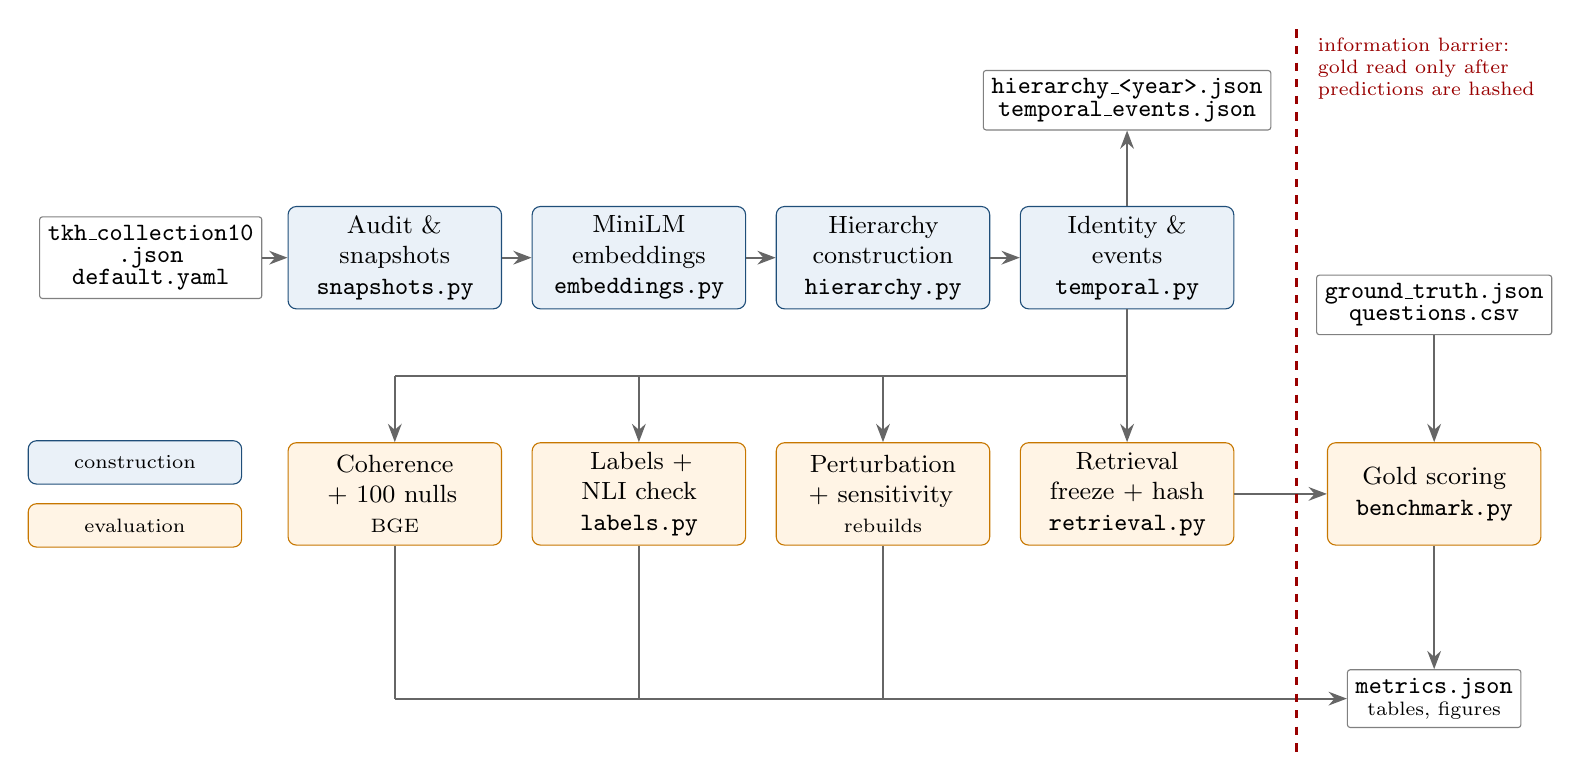
\begin{tikzpicture}[
  box/.style={draw=accent,fill=soft,rounded corners=3pt,align=center,font=\small,
              minimum width=2.7cm,text width=2.5cm,minimum height=1.3cm,inner sep=3pt},
  ebox/.style={draw=warnline,fill=warnsoft,rounded corners=3pt,align=center,font=\small,
              minimum width=2.7cm,text width=2.5cm,minimum height=1.3cm,inner sep=3pt},
  io/.style={draw=gray,fill=white,align=center,font=\scriptsize,rounded corners=1pt,inner sep=3pt},
  arr/.style={-{Stealth},thick,gray!80!black}]
  % ---- construction row (y = 0)
  \node[io]  (in)   at (0,0)    {\code{tkh\_collection10}\\\code{.json}\\\code{default.yaml}};
  \node[box] (aud)  at (3.1,0)    {Audit \&\\snapshots\\\scriptsize\code{snapshots.py}};
  \node[box] (emb)  at (6.2,0)    {MiniLM\\embeddings\\\scriptsize\code{embeddings.py}};
  \node[box] (hier) at (9.3,0)    {Hierarchy\\construction\\\scriptsize\code{hierarchy.py}};
  \node[box] (tmp)  at (12.4,0)   {Identity \&\\events\\\scriptsize\code{temporal.py}};
  \node[io]  (out)  at (12.4,2.0) {\code{hierarchy\_<year>.json}\\\code{temporal\_events.json}};
  % ---- evaluation row (y = -3)
  \node[ebox] (coh) at (3.1,-3)   {Coherence\\+ 100 nulls\\\scriptsize BGE};
  \node[ebox] (lab) at (6.2,-3)   {Labels +\\NLI check\\\scriptsize\code{labels.py}};
  \node[ebox] (per) at (9.3,-3)   {Perturbation\\+ sensitivity\\\scriptsize rebuilds};
  \node[ebox] (ret) at (12.4,-3)  {Retrieval\\freeze + hash\\\scriptsize\code{retrieval.py}};
  \node[ebox] (gold) at (16.3,-3) {Gold scoring\\\scriptsize\code{benchmark.py}};
  \node[io]  (gt)   at (16.3,-0.6) {\code{ground\_truth.json}\\\code{questions.csv}};
  \node[io]  (met)  at (16.3,-5.6) {\code{metrics.json}\\tables, figures};
  % ---- construction arrows
  \draw[arr] (in)--(aud); \draw[arr] (aud)--(emb); \draw[arr] (emb)--(hier);
  \draw[arr] (hier)--(tmp); \draw[arr] (tmp)--(out);
  % ---- bus from hierarchies to evaluation
  \draw[thick,gray!80!black] (tmp.south) -- (12.4,-1.5) -- (3.1,-1.5);
  \foreach \x/\n in {3.1/coh,6.2/lab,9.3/per,12.4/ret} \draw[arr] (\x,-1.5) -- (\n.north);
  % ---- evaluation arrows
  \draw[arr] (ret)--(gold); \draw[arr] (gt)--(gold); \draw[arr] (gold)--(met);
  \draw[thick,gray!80!black] (coh.south) -- (3.1,-5.6);
  \draw[thick,gray!80!black] (lab.south) -- (6.2,-5.6);
  \draw[thick,gray!80!black] (per.south) -- (9.3,-5.6);
  \draw[arr] (3.1,-5.6) -- (met.west);
  % ---- information barrier
  \draw[dashed,very thick,red!60!black] (14.55,2.9) -- (14.55,-6.3);
  \node[font=\scriptsize,red!60!black,align=left,anchor=west] at (14.7,2.4)
       {information barrier:\\gold read only after\\predictions are hashed};
  % ---- legend
  \node[box,minimum width=1.9cm,minimum height=0.55cm,font=\scriptsize] at (-0.2,-2.6) {construction};
  \node[ebox,minimum width=1.9cm,minimum height=0.55cm,font=\scriptsize] at (-0.2,-3.4) {evaluation};
\end{tikzpicture}}
\caption{End-to-end pipeline of \code{run\_all.py}. Construction (blue) never sees the
evaluation encoder or the benchmark. Retrieval predictions are written and hashed before
\code{benchmark.py} is imported and the ground truth is read.}
\label{fig:pipeline}
\end{figure}

The workflow proceeds in eight phases:

\begin{enumerate}
  \item \textbf{Source manifest.} Hash every source file, the configuration and the two
        annotation files. At the end of the run the hashes are recomputed, and the run is
        rejected if any source changed during execution.
  \item \textbf{Audit} (Gates A/B). Validate the schema, hash the inputs, detect
        anomalies, cut the four snapshots and write their statistics.
  \item \textbf{Construction embeddings.} Encode all 5{,}798 nodes once with MiniLM.
  \item \textbf{Build.} For each variant and each snapshot in time order, build the
        hierarchy (\cref{alg:tshc}) with the previous snapshot's hierarchy as history, then
        track identities and events and compute the transition metrics.
  \item \textbf{Coherence and labels.} Encode all nodes with BGE, compute coherence
        against nulls, and generate labels for every variant and snapshot.
  \item \textbf{Label NLI, perturbation, sensitivity.} Score labels, then rebuild the
        2026 hierarchies under edge deletion and parameter changes.
  \item \textbf{Retrieval.} Build documents, rank for all 18 questions $\times$ 5
        systems, write \code{predictions.json} and record its SHA-256 (Gate J).
  \item \textbf{Evaluation against gold.} Only now import \code{benchmark.py}, read the
        ground truth, score, check that the prediction hash is unchanged, write
        \code{metrics.json}, then draw figures.
\end{enumerate}

\subsection{Data loading and snapshots (\code{data.py}, \code{snapshots.py})}

\code{load\_graph} reads the JSON export and asserts the schema before anything else runs:
node and edge identifiers are unique, every node has a non-empty \code{surface\_form} and an
integer \code{first\_seen\_year}, every hyperedge refers only to existing nodes, has no
repeated member, and has arity at least 2. \code{manifest} records file sizes, SHA-256
hashes, JSON keys and record counts, and CSV delimiters. The benchmark CSV is
semicolon-separated, and the delimiter is detected, not assumed.

\code{snapshot(graph, year)} implements the visibility definition of \cref{sec:visibility}
in two filters: first the nodes with $\mathrm{first\_seen\_year}\le t$, then the hyperedges
that pass all three conditions. \code{anomalies} lists each inconsistent edge with its flags
and the year from which it becomes visible. \code{describe} produces the per-snapshot
statistics of \cref{tab:snapshots}: type counts, the arity histogram and growth. The test
\code{test\_snapshot\_defers\_article} checks that an edge whose asserting article is newer
than the snapshot is excluded.

\subsection{Embeddings with a content-addressed cache (\code{embeddings.py})}

The \code{Encoder} class wraps a Sentence-Transformers model on CPU with a pinned
revision. Every text is keyed by $\mathrm{SHA256}(\text{model name}+\text{revision}+\text{text})$
and stored as one \code{.npy} file. On each call, only uncached texts are encoded (in batches
of 64, with unit normalisation), and all vectors are then read back from the cache. The cache
therefore can never return a vector from a different model or revision, and an embedding
is computed once per unique text for the whole project. A separate-cache regeneration of all
18{,}008 embeddings reproduced the cached ones.

The \code{NLI} class loads the DeBERTa cross-encoder, checks that its label mapping is
exactly \{entailment, neutral, contradiction\}, and scores (premise, hypothesis) pairs in
batches of 16. Premise-only truncation (\code{truncation="only\_first"}) at 512 tokens
guarantees that the gloss is never cut. For every pair it records the untruncated token
count and a \code{truncated} flag, so any truncation is visible in the outputs.

\subsection{Hypergraph operations (\code{hypergraph.py})}

\begin{itemize}
  \item \code{collapse(edges, membership, year)} implements \cref{sec:collapse}. For each
        edge it counts endpoints per super-node, asserts that the counts sum to the
        original arity, and emits a record with \code{supernodes}, \code{multiplicity},
        \code{internal}, \code{original\_arity}, relation type, provenance and weight. It
        also accepts already-collapsed records, so collapse can be applied repeatedly
        across levels and still preserve the original arity.
  \item \code{project(edges)} builds the clique projection with weights $1/\binom r2$ and
        returns loss statistics (pair instances, unique pairs, collision pairs with their
        contributing edges).
  \item \code{fragmentation(edges, labels)} computes $F$ from scratch. It is not used by the
        optimiser, only by tests, as the reference for checking the incremental deltas.
\end{itemize}

\subsection{The hierarchy engine (\code{hierarchy.py})}

This is the core of the implementation. It deliberately receives only graph data,
construction vectors and a previous hierarchy. It has no access to the evaluation model or
the benchmark. A test (\code{test\_benchmark\_isolation\_source}) checks that the construction
modules' source contains no reference to the ground truth, the questions file or the benchmark
module.

\paragraph{\code{semantic\_links(X, k)}.}
Computes the full cosine similarity matrix $XX^\top$, masks the diagonal, and for each node
takes the $k$ most similar others using a \emph{stable} sort, so that ties break the same
way on every execution. Pairs are stored as ordered tuples $(\min,\max)$, which
symmetrises the relation.

\paragraph{The \code{Merger} class.}
It keeps, for every live cluster id:
\begin{center}
\begin{tabular}{ll}
\toprule
State & Used for\\
\midrule
\code{members}, \code{count} & membership and $n_C$\\
\code{sums} (float64 vector) & centroid $\mu_C=\text{sum}/n_C$ for $\Delta S$\\
\code{inc}: edge $\to$ multiplicity & $m_{e,C}$ for $\Delta F$\\
\code{previous}: old cluster $\to$ count & $c_{C,k}$ for $\Delta T$\\
\code{neighbors} & candidate graph adjacency\\
\bottomrule
\end{tabular}
\end{center}
In addition it precomputes one coefficient per hyperedge,
$w_e/(W\,r_e\log r_e)$, so each fragmentation delta is a short sum.

\begin{itemize}
  \item \code{delta(a, b)} evaluates \cref{eq:dF} and the $\Delta S$ and $\Delta T$
        formulas of \cref{sec:deltas}, always iterating over the \emph{smaller} of the two
        incidence or history maps.
  \item \code{push(a, b)} computes the delta and pushes $(\Delta,a,b)$ onto a binary heap.
        Ties are resolved by cluster ids, which makes the procedure fully deterministic.
  \item \code{run(budget)} executes the inner loop of \cref{alg:tshc}: pop until both
        clusters are alive, otherwise use the nearest-centroid fallback, then create a new
        cluster id and add up the sizes, vector sums, history counters and incidence
        counters of the two parents. The new cluster's neighbours are the union of the
        parents' neighbours, and each neighbour pair is pushed with its fresh delta.
\end{itemize}

Merging is cheap because every statistic is additive. Vector sums add, incidence
multiplicities add (\code{Counter} addition), and history counts add. No per-member work
is needed after a merge.

\paragraph{\code{build(snap, X, cfg, variant, previous)}.}
Sets up the variant (\cref{tab:variants}): $\alpha$, $\lambda$, which proposals to use,
and whether to use native edges, projected edges or none. It then runs three stages with
budgets 120, 40 and 12. Before each stage it:
\begin{enumerate}
  \item collapses the working edges onto the current clusters, so the new \code{Merger}
        starts from the actual multiplicities;
  \item loads the previous snapshot's partition \emph{at the same level} as the history map;
  \item creates a \code{Merger} over the current clusters and runs it to the budget.
\end{enumerate}
After each stage it re-indexes the live neighbour graph for the next stage (no new
proposal search) and stores the multiplicity-preserving collapse of the \emph{original}
hyperedges onto that level's super-nodes, with ids such as \code{2026\_L0\_3}. Merge
counts, fallbacks, candidate pair counts, the $\lambda$ used and the runtime are logged.

\paragraph{\code{validate}.}
Every hierarchy is checked before it is returned: each level contains every node exactly
once, each level respects its budget, every child has a single parent, and each parent's
members equal the union of its children's. A hierarchy that violates any invariant raises
an error and is never written.

\subsection{Temporal tracking (\code{temporal.py})}

\code{track(h, previous)} attaches the \code{supernodes} list to a hierarchy: one record per
cluster and level, with \code{id}, \code{level}, \code{parent\_id}, \code{child\_ids},
\code{member\_ids}, \code{size}, \code{persistent\_id}, and label and gloss fields that are
filled in later. At each level it builds the intersection and union matrices between old
and new clusters, computes Jaccard similarities, calls \code{linear\_sum\_assignment} on the
negated matrix to maximise similarity, and assigns persistent ids. It then walks the overlap
table and emits the events of \cref{tab:events}, keeping all non-zero overlaps (with
Jaccard and both overlap fractions) in \code{temporal\_overlap}. Finally it links parents and
children, and asserts that persistent ids are unique at every level.

\code{transition(old, new)} computes, for each level and on the nodes shared by both
snapshots, the ARI (scikit-learn), the VI (\cref{eq:vi}), the normalised VI
$\VI/(2\log n)$, and the \emph{lineage retention}: the fraction of shared nodes whose
persistent super-node id is unchanged. Tests check VI on empty and singleton inputs and its
invariance to relabelling.

\subsection{Labelling (\code{labels.py})}

\code{split\_members} performs the type-stratified, hash-ordered 70/30 split and asserts
that the two sets are disjoint and together cover the cluster. \code{generate} first asserts
that the snapshot contains only visible nodes and edges. For each level (0 and 1) it fits one
TF-IDF vocabulary on generation members only, then for each cluster computes the generation
centroid, representatives, phrase and gloss (\cref{sec:labels}). It writes the exact
generation input to \code{labels/inputs/<variant>/<id>.json} and returns a packet that also
holds the held-out text for evaluation. \code{evaluate\_labels} sends every evaluable packet to
the NLI scorer and computes the overclaim proxy and lexical support. Labels that cannot be
evaluated keep \code{null} values instead of being counted as successes. The test
\code{test\_nli\_proxy\_preserves\_unevaluable\_and\_neutral} checks this.

\subsection{Retrieval (\code{retrieval.py})}

\code{documents(snap, cfg)} builds the bounded context documents of
\cref{sec:retrieval-method}. It also records, for each document, the context node ids,
contributing hyperedge ids and source article ids (restricted to articles visible in the
snapshot), which are later used to score composite targets and source overlap.
\code{search(h, docs, X, q, beam)} runs either the flat scan (\code{beam=None}) or
\cref{alg:beam}. It returns the full ranking, the total comparisons split into cluster and
leaf work, and a complete trace of every comparison in order. The trace makes it possible to
compute ``comparisons until the first gold item was scored'' afterwards, without changing
the search.

\subsection{Evaluation orchestration (\code{evaluation.py})}

\paragraph{Sparse coherence.}
For cluster labels $\ell\in\{0,\dots,K-1\}^n$ and BGE matrix $Y$, a sparse $K\times n$
indicator matrix $M$ gives all cluster vector sums as $MY$ in one product. For unit vectors,
the mean cosine of the members to their normalised centroid equals $\|\sum_{v\in C}y_v\|/|C|$,
which is the length of the mean vector. Coherence is therefore
\[
\mathrm{coh}(C)=\frac{\big\|\sum_{v\in C}y_v\big\|}{|C|},\qquad
\text{macro}=\frac1K\sum_C\mathrm{coh}(C),\qquad
\text{size-weighted}=\frac{\sum_C\|\sum_{v\in C}y_v\|}{\sum_C|C|}.
\]
Singletons (coherence 1) are included in both the observation and the null, in the same way.
A test verifies that the sparse computation equals a naive indexed sum exactly.

\paragraph{Null model.}
\code{coherence} draws 100 null partitions with a fixed-seed generator (seed 42). Each is
created by permuting the cluster labels \emph{within each node type}. This keeps every
cluster's size and its exact type composition, and the code asserts both. Only
\emph{which} nodes of a given type sit in which cluster is randomised. The test is therefore
conditional and demanding: a cluster cannot beat the null merely because, for example, all
its members are datasets.

\paragraph{Perturbation and sensitivity.}
\code{execute\_evaluation} rebuilds the 2026 hierarchy for each variant after deleting a
seeded random 10\% of hyperedges, with the unperturbed 2024 hierarchy as history. The
sensitivity loop rebuilds the temporal 2026 hierarchy with one parameter changed at a time.
Both use the same \code{build} function as the main run.

\paragraph{Freeze, then score.}
After predictions are written, their SHA-256 is recorded in \code{gate\_J.json}. Only then
is \code{benchmark.py} imported. After scoring, the hash is recomputed and asserted equal,
and \code{evaluation\_independence.json} records the distinct models, the hash equality,
and the policies for labels, nulls and annotations.

\subsection{Benchmark scoring (\code{benchmark.py})}

This module is imported only after the freeze. It contains:

\begin{itemize}
  \item \code{support\_audit}: for each of the 63 expected-method occurrences, it looks for
        nodes whose normalised surface form (NFKC, casefolded, typographic hyphens unified)
        equals the target. If found, the status is \textbf{EXACT}. Otherwise an inspected
        evaluation-only annotation may assign \textbf{ALIAS} (explicit evidence of the same
        entity), \textbf{PARTIAL} (only part of the target's identity is present),
        \textbf{COMPOSITE} (the target is a bundle of components) or \textbf{ABSENT}.
  \item \code{align\_claims}: maps expected claims to claim nodes. Only exact text plus a
        resolved matching source article is accepted automatically. Semantic nearest
        neighbours are saved as \emph{proposals}, not accepted.
  \item \code{evaluate\_predictions}: scores each top-$k$ list. EXACT and ALIAS targets
        count only if the target node itself is ranked (\emph{direct identity}). A COMPOSITE
        target counts if all its components appear among the returned documents or their
        context. PARTIAL targets never count as complete recoveries but stay in the
        denominator.
\end{itemize}

\subsection{Determinism, tests and verification}

\paragraph{Determinism.}
All randomness comes from fixed seeds (null seed 42; perturbation seeds 11, 23, 37, 53, 71).
Sorting is stable with explicit tie-breakers, and label splits use hashes rather than a
random generator. Two complete fresh-output executions produced identical scientific
metrics, memberships, label probabilities and predictions.

\paragraph{Test suite.}
The 24 tests fall into four groups:
\begin{enumerate}
  \item \emph{Correctness of the optimiser}: incremental delta equals full objective (native
        and pairwise); the heap returns the exact current minimum; the disconnected-graph
        fallback preserves edge mass; laminar reproduction.
  \item \emph{Data semantics}: collapse multiplicities in parametrised cases; deferral of
        edges whose article is too new.
  \item \emph{Temporal bookkeeping}: birth/death and id references; merge/split thresholds;
        VI edge cases.
  \item \emph{Evaluation validity}: label split disjointness and visibility; NLI null
        handling; the all-leaf beam equals flat; null reproducibility; sparse coherence
        equals the naive sum; partial targets are not promoted; positive controls and
        context exclusion; a benchmark mutation does not change predictions; construction
        source isolation.
\end{enumerate}

\paragraph{Submission verification.}
\code{scripts/verify\_submission.py} re-reads the delivered outputs and checks structural
properties: the test report has at least 24 passes and no failures, hierarchy
parent/child consistency, collapse arities, event references, label split disjointness, NLI
probability sums, the expected number of perturbation rows and null replicates, 90
predictions, figures present. Optionally, it compares two complete output directories for
scientific equality.

\paragraph{Runtime.}
A complete run takes about 51 minutes on a laptop CPU (3{,}040~s measured). The main costs
are the 20 perturbation rebuilds and 7 sensitivity rebuilds of the 5{,}798-node graph, NLI
over 832 labels, and the 100 null replicates per level, snapshot and variant.

% ==================================================================
\section{Experimental Setup}
\label{sec:setup}
% ==================================================================

\subsection{Evaluation principles}

The task weights evaluation validity most heavily and warns against circularity. The
protocol follows five rules:

\begin{keybox}[Five validity rules]
\begin{enumerate}[leftmargin=*]
  \item \textbf{Different ruler.} Construction uses MiniLM. Coherence and retrieval use BGE,
        a different model family. The code asserts that the two model names differ.
  \item \textbf{Chance reference.} Every coherence value is compared with 100 null
        partitions that preserve cluster sizes and type composition.
  \item \textbf{Uncertainty, not points.} Perturbation stability uses five seeds with
        $t$-intervals. Temporal stability is reported for every transition and level.
  \item \textbf{Held-out label evidence.} Labels are checked only against members the
        labeller never saw.
  \item \textbf{Frozen predictions.} Retrieval outputs are hashed before any gold file is
        read, and nothing is tuned on the benchmark afterwards.
\end{enumerate}
\end{keybox}

\subsection{Intrinsic metrics}

\begin{description}[leftmargin=0.5cm,style=nextline]
  \item[Coherence (P3)] Size-weighted and macro BGE coherence at levels 0--2 for every
        variant and snapshot. Absolute effect over the null mean, standardised effect
        (effect / null SD), and empirical upper-tail $p$ with 100 replicates (floor
        $1/101=0.0099$). Tests are descriptive and not corrected for multiple comparisons.
  \item[Perturbation stability (P5)] At 2026, for each variant, delete $\mathrm{round}(0.1\times1429)=143$
        hyperedges with each of five seeds, rebuild with the unchanged 2024 history, and
        compute ARI to the unperturbed hierarchy at levels 0--2. Report mean, SD and the
        Student-$t$ 95\% interval ($n=5$). This measures sensitivity to \emph{current}
        evidence, not propagated historical damage.
  \item[Temporal stability (P5)] For the three real transitions (2020$\to$2022,
        2022$\to$2024, 2024$\to$2026) and three levels, on shared nodes: ARI, VI,
        normalised VI and lineage retention. The average over nine values is descriptive.
        The nine are not independent replications.
  \item[Label faithfulness (P6)] Overclaim proxy (fraction of evaluable glosses not entailed
        by held-out evidence), NLI class counts, lexical support and truncation counts,
        pooled over four snapshots, at levels 0 and 1.
\end{description}

\subsection{Extrinsic benchmark}

The benchmark has 18 questions: 14 of \textbf{Type A} (``Which methods, by Feb 2026, are best
suited for\dots'') with \code{expected\_methods}, and 4 of \textbf{Type B} with required
claims.

\paragraph{Target support audit.}
The gold target list is heterogeneous, so before scoring it was audited against the graph.
The 63 target occurrences (50 unique labels) break down as
\textbf{48 EXACT}, \textbf{1 ALIAS}, \textbf{11 PARTIAL}, \textbf{1 COMPOSITE} and
\textbf{2 ABSENT}. A basic normalised literal match finds 47 targets anywhere in the graph
but only 28 as \code{method}-type nodes, and 16 have no literal identity at all. Accepting
any node type for exact identity is therefore essential.

\paragraph{Metrics.}
\begin{itemize}
  \item \emph{Raw recall@$k$}: recovered targets / all 63 occurrences.
  \item \emph{Conditional (supported) recall@$k$}: recovered / 61 non-ABSENT occurrences.
  \item \emph{Work}: mean number of cosine comparisons per question.
  \item \emph{Comparisons to first target}: position in the scoring trace of the first
        EXACT/ALIAS target leaf, which depends on scan order.
  \item \emph{Type-B claim recovery} for aligned claims, and \emph{source recovery}: the
        fraction of expected source articles among the sources of the returned documents.
        Source recovery is a coarse signal, not claim correctness.
\end{itemize}
$k\in\{10,25\}$. The systems are the flat baseline and beams 1/3/5/10 (beam 3 primary).

\paragraph{Claim alignment.}
Of 224 expected claims (188 Type-A method claims and 36 Type-B required claims), only
\textbf{1} could be aligned defensibly to a claim node: exact text plus a matching source,
or an explicitly inspected annotation. All the others are marked
\code{NOT\_EVALUABLE\_ALIGNMENT} instead of being guessed. The one accepted alignment
(Q18.C16) was annotated \emph{post hoc}, after the frozen results had been inspected, so it
is not independent validation.

\subsection{Sensitivity protocol}
\label{sec:sens-protocol}

With the 2024 temporal hierarchy fixed as history, the 2026 temporal hierarchy is rebuilt
with one parameter changed at a time: $\alpha\in\{0.25,0.75\}$, $\lambda\in\{0,0.1,0.4\}$ and
$k\in\{5,20\}$. Each rebuild is compared with the primary hierarchy by ARI. This is a study
of how much the results depend on each parameter. It is \emph{not} parameter selection, and
the primary values were fixed before any results were seen.

% ==================================================================
\section{Results}
\label{sec:results}
% ==================================================================

All numbers in this section were regenerated by one complete run of the clean
implementation and read from \code{outputs/metrics.json} and \code{outputs/tables/}. A
second fresh-output run reproduced them exactly.

\subsection{Overview}

\begin{table}[!htbp]
\centering
\caption{Headline comparison of the four variants. Coherence: 2026 size-weighted BGE
coherence. Temporal ARI: mean over three transitions and three levels (descriptive).
Perturbation: five-seed mean $\pm$ SD of ARI to the unperturbed 2026 hierarchy.}
\label{tab:headline}
\small
\begin{tabular}{lccccccc}
\toprule
& \multicolumn{3}{c}{Coherence (2026)} & Temporal & \multicolumn{3}{c}{Perturbation ARI}\\
\cmidrule(lr){2-4}\cmidrule(lr){6-8}
Variant & L0 & L1 & L2 & ARI & L0 & L1 & L2\\
\midrule
semantic & \textbf{0.8240} & \textbf{0.8407} & \textbf{0.8608} & 0.4667 & $1.000\pm0.000$ & $1.000\pm0.000$ & $1.000\pm0.000$\\
pairwise & 0.7978 & 0.8008 & 0.8073 & 0.6897 & $0.679\pm0.028$ & $0.637\pm0.047$ & $0.565\pm0.020$\\
static   & 0.8075 & 0.8120 & 0.8208 & 0.7247 & $0.780\pm0.019$ & $0.753\pm0.036$ & $0.765\pm0.042$\\
temporal & 0.8029 & 0.8108 & 0.8205 & \textbf{0.8924} & $0.781\pm0.115$ & $0.818\pm0.099$ & $0.869\pm0.094$\\
\bottomrule
\end{tabular}
\end{table}

The semantic-only perturbation ARI of exactly 1 is not robustness. That variant ignores
hyperedges entirely, so deleting edges cannot change it. The value measures blindness to
edges.

\subsection{Coherence against the null model (P3)}

\begin{table}[!htbp]
\centering
\caption{2026 size-weighted coherence versus 100 type- and size-preserving null partitions.
All empirical $p$-values equal the resolution floor $1/101$: no null replicate reached the
observed value.}
\label{tab:coherence}
\small
\begin{tabular}{llccccc}
\toprule
Variant & Level & Observed & Null mean & Abs.\ effect & Std.\ effect & $p$\\
\midrule
\multirow{3}{*}{semantic} & 0 & 0.8240 & 0.8108 & 0.0132 & 99.2 & 0.0099\\
 & 1 & 0.8407 & 0.8136 & 0.0271 & 189.1 & 0.0099\\
 & 2 & 0.8608 & 0.8183 & 0.0425 & 281.3 & 0.0099\\
\midrule
\multirow{3}{*}{pairwise} & 0 & 0.7978 & 0.7955 & 0.0023 & 14.7 & 0.0099\\
 & 1 & 0.8008 & 0.7970 & 0.0038 & 24.7 & 0.0099\\
 & 2 & 0.8073 & 0.8006 & 0.0067 & 39.9 & 0.0099\\
\midrule
\multirow{3}{*}{static} & 0 & 0.8075 & 0.8048 & 0.0026 & 15.5 & 0.0099\\
 & 1 & 0.8120 & 0.8063 & 0.0057 & 33.1 & 0.0099\\
 & 2 & 0.8208 & 0.8103 & 0.0104 & 62.6 & 0.0099\\
\midrule
\multirow{3}{*}{temporal} & 0 & 0.8029 & 0.7996 & 0.0033 & 22.4 & 0.0099\\
 & 1 & 0.8108 & 0.8046 & 0.0062 & 35.7 & 0.0099\\
 & 2 & 0.8205 & 0.8092 & 0.0113 & 70.4 & 0.0099\\
\bottomrule
\end{tabular}
\end{table}

\begin{figure}[!htbp]
\centering
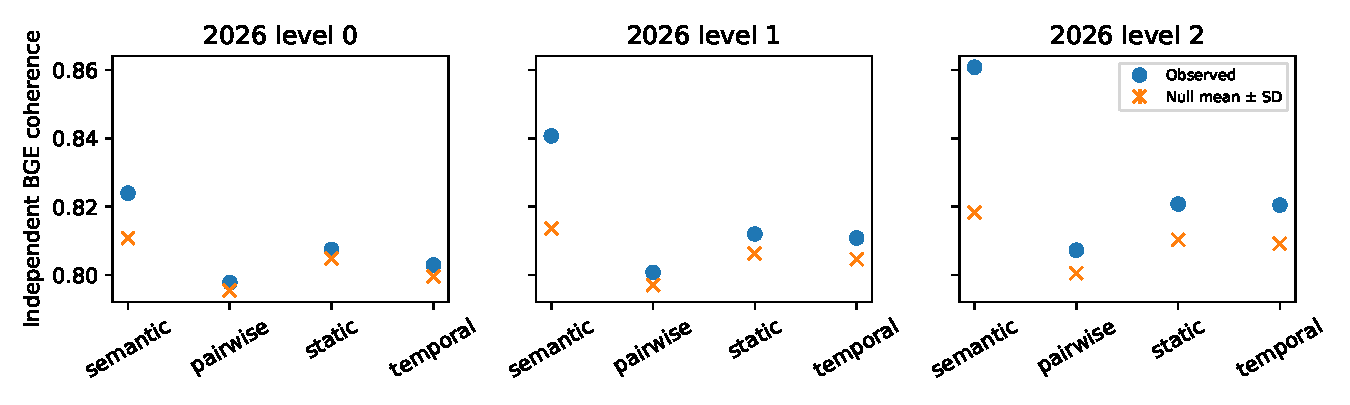
\includegraphics[width=\linewidth]{coherence_vs_null.pdf}
\caption{Independent BGE coherence (dots) against the null mean $\pm$ SD (crosses) for the
2026 snapshot. The null SD is so small that its error bars are invisible.}
\label{fig:coherence}
\end{figure}

\paragraph{Observations.}
\begin{enumerate}
  \item \textbf{Every variant beats chance at every level.} All 12 comparisons have
        $p=1/101$. The \emph{independent} encoder confirms that the clusters group
        semantically related nodes beyond what cluster size and type composition explain.
  \item \textbf{The absolute effects are small.} For the temporal variant they are
        0.0033, 0.0062 and 0.0113 cosine at L0, L1 and L2. Standardised effects of 22--70
        look large only because the null distribution is very narrow (SD $\approx$ 0.00015).
        They should not be read as large practical effects.
  \item \textbf{Finer levels are more coherent}, as expected: smaller clusters are more
        homogeneous.
  \item \textbf{Semantic-only is the most coherent}, with effects roughly four times
        those of the temporal variant. It optimises meaning alone, so this is expected. That
        the gap survives an independent encoder shows it is a real property, not
        self-grading.
  \item \textbf{Pairwise is the least coherent} of all variants at every level.
\end{enumerate}

The effect is stable across snapshots (\cref{tab:coh-years}): the temporal variant beats
its null at every level of every year.

\begin{table}[!htbp]
\centering
\caption{Temporal variant: size-weighted coherence and absolute effect over the null in every
snapshot (all $p=0.0099$).}
\label{tab:coh-years}
\small
\begin{tabular}{lcccccc}
\toprule
& \multicolumn{2}{c}{Level 0} & \multicolumn{2}{c}{Level 1} & \multicolumn{2}{c}{Level 2}\\
\cmidrule(lr){2-3}\cmidrule(lr){4-5}\cmidrule(lr){6-7}
Year & Observed & Effect & Observed & Effect & Observed & Effect\\
\midrule
2020 & 0.8078 & 0.0058 & 0.8191 & 0.0098 & 0.8354 & 0.0146\\
2022 & 0.8072 & 0.0034 & 0.8172 & 0.0073 & 0.8316 & 0.0129\\
2024 & 0.8077 & 0.0033 & 0.8165 & 0.0070 & 0.8276 & 0.0127\\
2026 & 0.8029 & 0.0033 & 0.8108 & 0.0062 & 0.8205 & 0.0113\\
\bottomrule
\end{tabular}
\end{table}

\subsection{Temporal stability across real snapshots (P5)}

\begin{table}[!htbp]
\centering
\caption{Cross-snapshot ARI on shared nodes, for every transition and level.}
\label{tab:temporal-ari}
\small
\begin{tabular}{llccc c}
\toprule
Variant & Transition & L0 & L1 & L2 & Mean\\
\midrule
\multirow{3}{*}{semantic} & 2020$\to$2022 & 0.396 & 0.424 & 0.664 & \multirow{3}{*}{0.467}\\
 & 2022$\to$2024 & 0.394 & 0.384 & 0.521 & \\
 & 2024$\to$2026 & 0.421 & 0.455 & 0.539 & \\
\midrule
\multirow{3}{*}{pairwise} & 2020$\to$2022 & 0.863 & 0.843 & 0.789 & \multirow{3}{*}{0.690}\\
 & 2022$\to$2024 & 0.551 & 0.446 & 0.514 & \\
 & 2024$\to$2026 & 0.739 & 0.759 & 0.702 & \\
\midrule
\multirow{3}{*}{static} & 2020$\to$2022 & 0.545 & 0.860 & 0.855 & \multirow{3}{*}{0.725}\\
 & 2022$\to$2024 & 0.682 & 0.556 & 0.617 & \\
 & 2024$\to$2026 & \textbf{0.765} & \textbf{0.789} & \textbf{0.853} & \\
\midrule
\multirow{3}{*}{temporal} & 2020$\to$2022 & \textbf{0.962} & \textbf{0.964} & \textbf{0.960} & \multirow{3}{*}{\textbf{0.892}}\\
 & 2022$\to$2024 & \textbf{0.942} & \textbf{0.948} & \textbf{0.942} & \\
 & 2024$\to$2026 & 0.760 & 0.782 & 0.772 & \\
\bottomrule
\end{tabular}
\end{table}

\begin{figure}[!htbp]
\centering
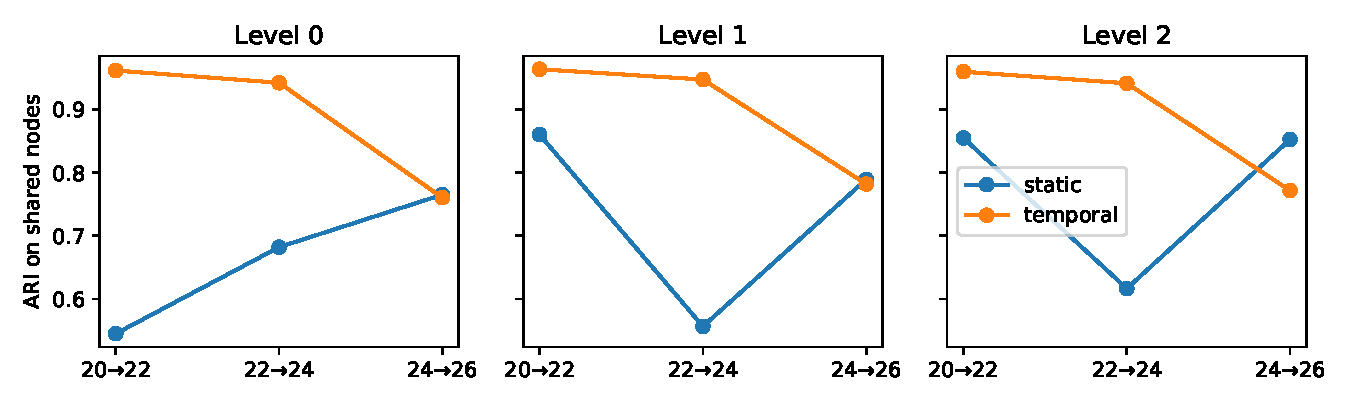
\includegraphics[width=\linewidth]{temporal_stability.pdf}
\caption{Cross-snapshot ARI of the static and temporal native variants per level.}
\label{fig:temporal}
\end{figure}

\begin{table}[!htbp]
\centering
\caption{Static versus temporal: normalised VI (lower is more stable) and lineage retention
(fraction of shared nodes keeping their persistent super-node id).}
\label{tab:vi-lineage}
\small
\begin{tabular}{llcccccc}
\toprule
& & \multicolumn{3}{c}{Normalised VI} & \multicolumn{3}{c}{Lineage retention}\\
\cmidrule(lr){3-5}\cmidrule(lr){6-8}
Transition & Variant & L0 & L1 & L2 & L0 & L1 & L2\\
\midrule
\multirow{2}{*}{2020$\to$2022} & static & 0.058 & 0.031 & 0.030 & 0.797 & 0.901 & 0.898\\
 & temporal & \textbf{0.007} & \textbf{0.008} & \textbf{0.008} & \textbf{0.985} & \textbf{0.981} & \textbf{0.981}\\
\midrule
\multirow{2}{*}{2022$\to$2024} & static & 0.051 & 0.073 & 0.072 & 0.845 & 0.757 & 0.754\\
 & temporal & \textbf{0.011} & \textbf{0.012} & \textbf{0.011} & \textbf{0.978} & \textbf{0.970} & \textbf{0.969}\\
\midrule
\multirow{2}{*}{2024$\to$2026} & static & 0.043 & 0.047 & 0.045 & 0.886 & 0.850 & 0.838\\
 & temporal & \textbf{0.024} & \textbf{0.023} & \textbf{0.021} & \textbf{0.895} & \textbf{0.897} & \textbf{0.893}\\
\bottomrule
\end{tabular}
\end{table}

\paragraph{Observations.}
\begin{itemize}
  \item Temporal regularisation raises the mean ARI from \textbf{0.725} (static) to
        \textbf{0.892}, and in the first two transitions it keeps about 97--98\% of shared nodes
        in the same lineage.
  \item \textbf{Qualification:} in the last transition (2024$\to$2026), the temporal ARI is
        \emph{slightly below} static at all three levels (e.g.\ L2: 0.772 vs 0.853). The
        normalised VI and lineage retention still favour the temporal variant at all three
        levels. The conclusion about the final transition therefore depends on which stability
        metric is used. ARI is pair-based and dominated by the giant cluster, whereas VI is
        information-based.
  \item Semantic-only is the least stable (0.467), despite being blind to edges. With no
        structure and no history, small changes in the $k$NN graph as nodes are added
        reshuffle the clusters.
\end{itemize}

\paragraph{Event log.}
\Cref{tab:event-counts} counts the events. Deaths never occur because snapshots are
cumulative and every old member is still present. The temporal variant turns most matched
super-nodes into continuations or growth, has the fewest merges and splits, and has far
fewer births than static or pairwise.
Semantic-only is dominated by merges and splits, which is consistent with its low ARI.

\begin{table}[!htbp]
\centering
\caption{Temporal events per transition (all levels 0--2 together; 172 super-nodes per
snapshot). Deaths: 0 for all variants and transitions.}
\label{tab:event-counts}
\small
\begin{tabular}{llccccc}
\toprule
Variant & Transition & Birth & Continuation & Growth & Merge & Split\\
\midrule
\multirow{3}{*}{semantic} & 20$\to$22 & 5 & 15 & 140 & 85 & 89\\
 & 22$\to$24 & 6 & 2 & 155 & 108 & 107\\
 & 24$\to$26 & 2 & 4 & 154 & 107 & 95\\
\midrule
\multirow{3}{*}{pairwise} & 20$\to$22 & 53 & 89 & 24 & 3 & 7\\
 & 22$\to$24 & 109 & 26 & 19 & 4 & 9\\
 & 24$\to$26 & 31 & 42 & 31 & 7 & 9\\
\midrule
\multirow{3}{*}{static} & 20$\to$22 & 52 & 78 & 40 & 13 & 7\\
 & 22$\to$24 & 78 & 29 & 52 & 19 & 13\\
 & 24$\to$26 & 15 & 63 & 67 & 23 & 30\\
\midrule
\multirow{3}{*}{temporal} & 20$\to$22 & 17 & 98 & 56 & 2 & 3\\
 & 22$\to$24 & 19 & 63 & 84 & 11 & 6\\
 & 24$\to$26 & 7 & 84 & 77 & 9 & 8\\
\bottomrule
\end{tabular}
\end{table}

Concrete examples from the primary run: \code{L0\_2020\_0001} continues with all 128 of its
members, and \code{L0\_2020\_0000} keeps all of its 941 old members while growing. Of the
twelve 2026 level-0 super-nodes, eleven carry persistent ids born in 2020, and one
(\code{L0\_2024\_0006}, labelled ``mlips'') was born in 2024.

\subsection{Stability under perturbation (P5)}

\begin{table}[!htbp]
\centering
\caption{ARI between the 2026 hierarchy rebuilt after deleting 10\% of hyperedges (143 edges)
and the unperturbed hierarchy. Five seeds; Student-$t$ 95\% intervals.}
\label{tab:perturb}
\small
\begin{tabular}{lccc}
\toprule
Variant & L0 & L1 & L2\\
\midrule
semantic & 1.000 [1.000, 1.000] & 1.000 [1.000, 1.000] & 1.000 [1.000, 1.000]\\
pairwise & 0.679 [0.645, 0.714] & 0.637 [0.579, 0.695] & 0.565 [0.541, 0.589]\\
static   & 0.780 [0.757, 0.803] & 0.753 [0.708, 0.797] & 0.765 [0.713, 0.818]\\
temporal & 0.781 [0.639, 0.923] & 0.818 [0.695, 0.940] & 0.869 [0.751, 0.986]\\
\bottomrule
\end{tabular}
\end{table}

\begin{figure}[!htbp]
\centering
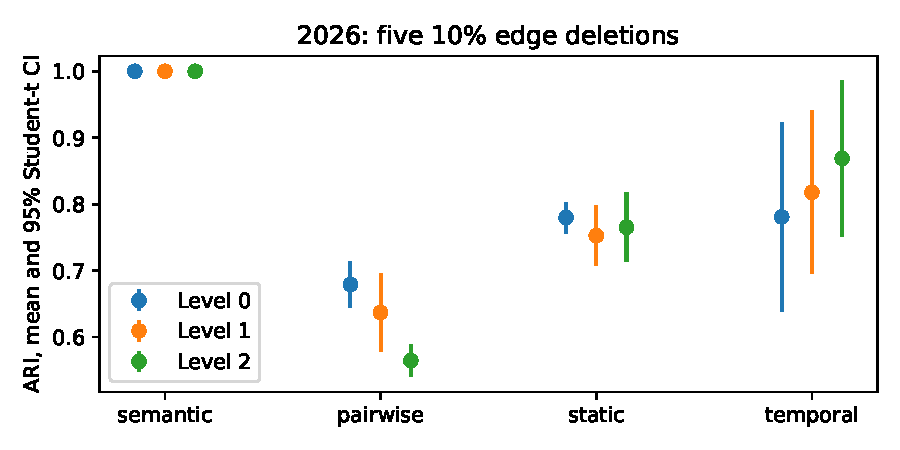
\includegraphics[width=0.9\linewidth]{perturbation_stability.pdf}
\caption{Perturbation ARI with 95\% confidence intervals over five deletion seeds.}
\label{fig:perturb}
\end{figure}

The native variants are clearly more robust than the pairwise projection. The pairwise
intervals lie entirely below the static intervals at all three levels, and below the temporal
intervals at L1 and L2: the projection's clusters change more when relations are removed. The temporal variant has the highest means at L1 and L2 but also the widest
intervals (SD about 0.1). Its intervals overlap the static ones substantially, so with five
seeds \textbf{no robustness advantage of temporal over static can be claimed}.

\subsection{Label faithfulness (P6)}

\begin{table}[!htbp]
\centering
\caption{Label faithfulness pooled over the four snapshots. Overclaim = fraction of evaluable
glosses not entailed by held-out evidence (lower is better), with $t$-interval.
Truncated = labels with character or token truncation of the premise.}
\label{tab:labels}
\small
\begin{tabular}{llrrrcrrrr}
\toprule
Variant & Lvl & Labels & Eval. & N/A & Overclaim [95\% CI] & Ent. & Neu. & Con. & Trunc.\\
\midrule
semantic & 0 & 48 & 44 & 4 & 0.386 [0.237, 0.536] & 27 & 12 & 5 & 27\\
semantic & 1 & 160 & 152 & 8 & 0.322 [0.247, 0.398] & 103 & 29 & 20 & 42\\
pairwise & 0 & 48 & 37 & 11 & 0.405 [0.239, 0.571] & 22 & 10 & 5 & 6\\
pairwise & 1 & 160 & 46 & 114 & 0.457 [0.307, 0.606] & 25 & 11 & 10 & 6\\
static & 0 & 48 & 44 & 4 & \textbf{0.136} [0.031, 0.242] & 38 & 5 & 1 & 14\\
static & 1 & 160 & 124 & 36 & 0.371 [0.285, 0.457] & 78 & 29 & 17 & 13\\
temporal & 0 & 48 & 44 & 4 & 0.318 [0.175, 0.461] & 30 & 11 & 3 & 16\\
temporal & 1 & 160 & 130 & 30 & \textbf{0.308} [0.227, 0.388] & 90 & 26 & 14 & 15\\
\bottomrule
\end{tabular}
\end{table}

Over both levels, the primary temporal variant has 208 labels, 174 of them evaluable, with
120 entailed, 37 neutral and 17 contradicted, for an overall overclaim proxy of
$54/174=0.310$. The picture is \textbf{mixed}. Static is best at L0 (0.136) and temporal is best
at L1 (0.308). Pairwise leaves 114 of 160 L1 labels unevaluable, because its many tiny and
singleton clusters have no held-out evidence. Lexical support (the fraction of label words
found in held-out text) is 0.87 for temporal L0 and 0.71 for L1.

\begin{table}[!htbp]
\centering
\caption{The twelve level-0 super-nodes of the primary (temporal) 2026 hierarchy.
``---'' means that no representative name was short enough ($\le$100 characters) to quote.}
\label{tab:l0labels}
\small
\begin{tabularx}{\linewidth}{lrlX}
\toprule
Persistent id & Size & Label & Representatives quoted in the gloss\\
\midrule
L0\_2020\_0000 & 3{,}765 & materials & Embedded Atom Neural Network Potentials; Slow, trial-and-error materials discovery\\
L0\_2020\_0007 & 603 & feature & Weak-scaling evaluation; AdamW optimizer\\
L0\_2020\_0005 & 402 & layer & Elemental embedding; Element-expert pairs\\
L0\_2020\_0011 & 259 & prediction & Element-wise phonon energy prediction; phonon property prediction\\
L0\_2020\_0001 & 186 & carbon & Accurate data-driven interatomic potentials; accuracy-cost tradeoff\\
L0\_2020\_0002 & 169 & Scientific evidence & --- (fallback label)\\
L0\_2020\_0003 & 130 & al & Cen et al.; Maruf et al.\\
L0\_2020\_0004 & 72 & descriptor & conservative prediction mode; direct prediction mode\\
L0\_2020\_0008 & 72 & carbon & computational materials modeling; Crystal structure property prediction\\
L0\_2024\_0006 & 66 & mlips & ---\\
L0\_2020\_0010 & 49 & parallel & parallelization of GNN-based interatomic potentials; scalable parallel computation\\
L0\_2020\_0006 & 25 & jarvis & JARVIS-Tools; JARVIS-FF\\
\bottomrule
\end{tabularx}
\end{table}

\Cref{tab:l0labels} shows why the numbers should be read with care. Several labels are
conservative but too generic to navigate by (``materials'', ``feature'', ``layer''). Two
L0 clusters share the label ``carbon''. One is the fallback. One (``al'') comes from
citation-style names such as ``Cen et al.'', which are typed \code{cited\_work} rather than
\code{author} and therefore escape the author filter. A generic gloss about ``evidence concerning
materials'' is easy to entail, so a low overclaim rate can reward vagueness.

\subsection{Extrinsic evaluation: coarse-to-fine retrieval}

\begin{table}[!htbp]
\centering
\caption{Retrieval for Type-A questions (63 target occurrences, 61 supported). Recall is
identical at $k=10$ and $k=25$. Work = mean cosine comparisons per question; reduction is
relative to flat. First hit = median comparisons until the first EXACT/ALIAS target is scored
(misses excluded); No hit = questions where no target was ever scored.}
\label{tab:retrieval}
\small
\setlength{\tabcolsep}{4pt}
\begin{tabular}{lcccccccc}
\toprule
System & Recov. & Raw & Cond. & Work & Reduct. & First & No & Source rec.\\
 & & rec. & rec. & & & hit & hit & @10 / @25\\
\midrule
flat   & 0/63 & 0.000 & 0.000 & 5{,}480.0 & ---     & 85  & 2  & 0.750 / 0.750\\
beam1  & 0/63 & 0.000 & 0.000 & 476.9     & 91.3\%  & 110 & 12 & 0.771 / 0.771\\
\textbf{beam3} & 0/63 & 0.000 & 0.000 & 1{,}711.7 & 68.8\% & 136 & 7 & 0.750 / 0.833\\
beam5  & 0/63 & 0.000 & 0.000 & 2{,}508.2 & 54.2\%  & 142 & 3  & 0.750 / 0.833\\
beam10 & 0/63 & 0.000 & 0.000 & 3{,}030.9 & 44.7\%  & 171 & 2  & 0.750 / 0.750\\
\bottomrule
\end{tabular}
\end{table}

\begin{figure}[!htbp]
\centering
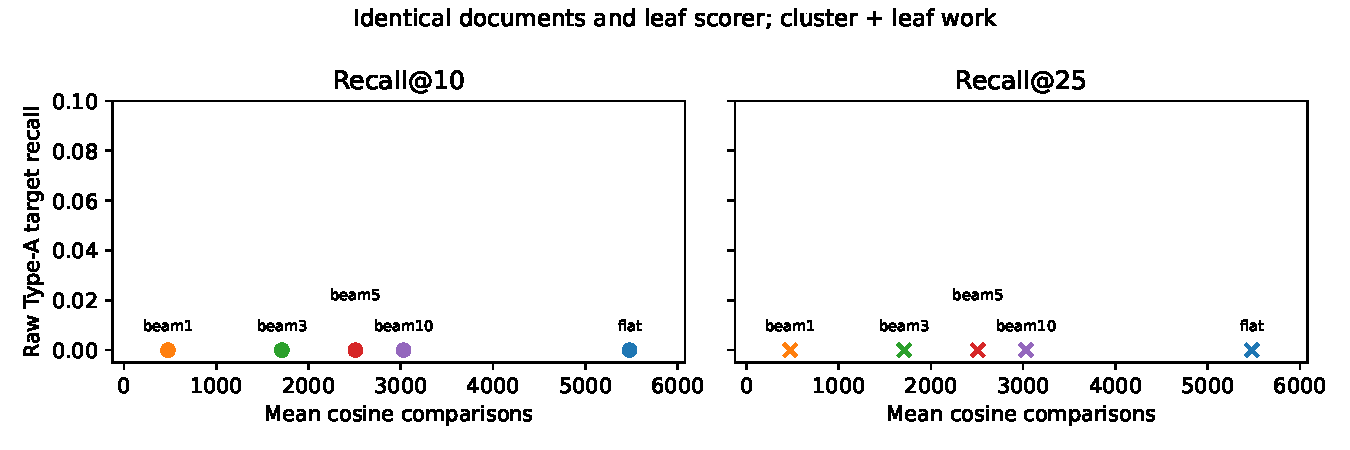
\includegraphics[width=\linewidth]{retrieval_work_tradeoff.pdf}
\caption{Retrieval work against raw Type-A target recall. All systems recover zero targets,
while the work varies by an order of magnitude.}
\label{fig:retrieval}
\end{figure}

\begin{cautionbox}[Negative result]
Under the declared recovery rule (the gold method node itself must be ranked in the top $k$),
\textbf{no system recovers any Type-A target}: not the flat baseline, and not any beam. The
hierarchy reduces comparison work by 45--91\%, but there is no recall to preserve. The
extrinsic evaluation therefore does \emph{not} show that the hierarchy helps the downstream
task.
\end{cautionbox}

\paragraph{Is the evaluator broken?}
A zero result could come from a bug in scoring, so two controls were run:
\begin{enumerate}
  \item \textbf{Positive control.} For all 49 EXACT/ALIAS target instances, the mapped node
        was forced into first place of an otherwise unchanged ranking. The evaluator recovered
        \textbf{49/49}. The scorer does count real hits.
  \item \textbf{Rank inspection.} The best flat ranks of the gold nodes show a genuine ranking
        failure: MatterSim (Q12) is at rank 31, DeepH-E3 (Q3) at 57, xDeepH at 106, and
        ``GNN stress fields'' (Q8) at 287. For Q1, the widely known potentials rank very low:
        M3GNet 880, CHGNet 1{,}340, NequIP 1{,}536, MACE 5{,}437 of 5{,}480.
\end{enumerate}
Meanwhile the top flat results are topically relevant. For Q3 the top three are problem
and task nodes about twisted van der Waals materials and Hamiltonian learning whose context
\emph{mentions} DeepH-E3. For Q8 they are fracture-prediction problems whose context contains
the ConvLSTM model. The relevant evidence is found, but the exact method identity is not
ranked.

\paragraph{Type-B questions.}
Only one of 36 Type-B required claims could be aligned, and it was recovered in 0 of 10
system/cutoff evaluations. The coarse source signal is better: at $k=10$, flat and beam3 both
return documents from 75\% of the expected source articles on average (four questions), and
beam3 reaches 83\% at $k=25$. This measures topical overlap, not claim correctness.

\subsection{Parameter sensitivity}
\label{sec:sens}

\begin{table}[!htbp]
\centering
\caption{One-at-a-time sensitivity of the 2026 temporal hierarchy (2024 history fixed). ARI
vs primary: agreement with the primary hierarchy. Coh.\ L0: size-weighted BGE coherence.
ARI 24$\to$26: temporal stability of the rebuilt hierarchy at L0. The primary setting is
shown in bold.}
\label{tab:sens}
\small
\begin{tabular}{lcccccc}
\toprule
Parameter & Value & \multicolumn{3}{c}{ARI vs primary} & Coh.\ L0 & ARI 24$\to$26 (L0)\\
\cmidrule(lr){3-5}
& & L0 & L1 & L2 & & \\
\midrule
\multirow{3}{*}{$\alpha$} & 0.25 & 0.698 & 0.814 & 0.821 & 0.7987 & 0.733\\
 & \textbf{0.50} & 1 & 1 & 1 & 0.8029 & 0.760\\
 & 0.75 & 0.617 & 0.693 & 0.699 & 0.8101 & 0.964\\
\midrule
\multirow{4}{*}{$\lambda$} & 0 & 0.376 & 0.493 & 0.648 & 0.8075 & 0.391\\
 & 0.1 & 0.760 & 0.838 & 0.849 & 0.8067 & 0.881\\
 & \textbf{0.2} & 1 & 1 & 1 & 0.8029 & 0.760\\
 & 0.4 & 0.749 & 0.773 & 0.775 & 0.8095 & 0.985\\
\midrule
\multirow{3}{*}{$k$} & 5 & 0.934 & 0.991 & 0.998 & 0.8027 & 0.750\\
 & \textbf{10} & 1 & 1 & 1 & 0.8029 & 0.760\\
 & 20 & 0.950 & 0.997 & 0.999 & 0.8031 & 0.760\\
\bottomrule
\end{tabular}
\end{table}

$\alpha$ and $\lambda$ change the memberships substantially, while the number of neighbours
$k$ hardly matters (ARI $\ge0.93$). Two results stand out and are reported although they
flatter alternatives to the primary configuration. First, $\alpha=0.75$ (more weight on
meaning) gives both higher coherence and a much higher last-transition ARI. Second, the
relationship with $\lambda$ is not monotone: $\lambda=0.1$ and $0.4$ both give higher
last-transition ARI than $\lambda=0.2$. These are single-snapshot diagnostics, and switching
to them after seeing the results would be outcome-driven tuning. The primary configuration
was therefore not changed.

\subsection{Structure of the hierarchy}

\begin{table}[!htbp]
\centering
\caption{Largest cluster size per level (2026), and share of original hyperedges that become
internal (all endpoints in one super-node) at each level of the primary hierarchy.}
\label{tab:sizes}
\small
\begin{tabular}{lccc}
\toprule
Variant & Largest L0 & Largest L1 & Largest L2\\
\midrule
semantic & 1{,}601 & 447 & 307\\
pairwise & 5{,}157 & 5{,}021 & 4{,}769\\
static & 3{,}535 & 3{,}334 & 2{,}880\\
temporal & 3{,}765 & 3{,}043 & 2{,}615\\
\bottomrule
\end{tabular}
\hspace{0.6cm}
\begin{tabular}{lcc}
\toprule
Level & Internal edges & Share\\
\midrule
L2 (120) & 1{,}269 / 1{,}429 & 88.8\%\\
L1 (40) & 1{,}293 / 1{,}429 & 90.5\%\\
L0 (12) & 1{,}318 / 1{,}429 & 92.2\%\\
\bottomrule
\end{tabular}
\end{table}

All structure-aware variants produce a \textbf{dominant cluster}. In the primary 2026
hierarchy one L0 super-node holds 3{,}765 of 5{,}798 nodes (65\%), and it grew from 941 nodes
in 2020 through 1{,}353 and 2{,}429. Most hyperedges end up entirely inside one super-node,
even at the finest level (88.8\%). At L0, only 111 hyperedges remain between super-nodes, of
which 24 span three or more.

\subsection{Runtime}

Construction times for the full four-snapshot sequence were 9~s (semantic), 128~s (static),
168~s (pairwise) and 199~s (temporal). The largest single build (temporal, 2026) took 133~s.
The complete workflow, including all evaluation, took 3{,}040~s ($\approx$51 minutes) on CPU.

% ==================================================================
\section{Discussion}
\label{sec:discussion}
% ==================================================================

\subsection{RQ1: combining structure and meaning}

The joint objective works as designed in the formal sense. It is explicit, it is optimised
exactly in each greedy step (verified against the full objective), it guarantees laminarity and
budgets, and the native hyperedge representation it optimises is the one it outputs. The
independent evaluation also shows that structure matters: the native variants are more robust
to edge deletion than the projection and more stable over time than the semantic-only
variant.

The trade-off is visible in the results. Every structure-aware variant is less coherent than
semantic-only, so the structural term pulls clusters away from pure meaning. The dominant
cluster explains much of this. Many small, cheap merges reduce fragmentation, and the graph
contains hub nodes (broad tasks, frequently used techniques) that connect many hyperedges.
Merging along those hubs lowers $F$ substantially. $F$ ranges over $[0,1]$ while $S$ is capped at
$0.25$, so with $\alpha=0.5$ the fragmentation term has more realised influence than its nominal
weight suggests. The sensitivity study supports this reading: raising $\alpha$ to 0.75 increases
coherence. A size or balance penalty was deliberately \emph{not} added after inspecting the
outputs, because that would have been outcome-driven redesign.

The pairwise baseline is the clearest confirmation that the projection loses something. It has
the lowest coherence, the lowest perturbation robustness,
the most extreme giant cluster (5{,}157 nodes at L0) and the most unevaluable labels. Its
perturbation intervals lie below those of the native variants.

\subsection{RQ2: the price and value of temporal regularisation}

Temporal regularisation delivers the continuity it was designed for. Mean ARI rises from 0.725
to 0.892, VI falls in every transition and level, and lineage retention reaches 97--98\% in the
first two transitions. The cost in coherence is small: mean 2026 coherence across levels falls
from 0.8134 (static) to 0.8114 (temporal), a difference of 0.002 cosine. On this corpus the
trade is favourable.

Two qualifications apply. In the last transition, ARI favours static while VI and lineage
favour temporal, so the claim ``temporal is more stable'' holds on average and by the
information-theoretic metrics, not at every transition by every metric. And the $\lambda$
sensitivity is non-monotone, which suggests that the greedy path interacts with the regulariser
in ways that a single $\lambda$ does not fully control.

\subsection{RQ3: coherence beyond chance}

Yes, and the result is robust, because it is measured with an encoder that played no part in
construction, against nulls that preserve cluster sizes and type composition. The effects are
small in absolute terms, which is itself informative. Once type composition is fixed, much of
the apparent coherence of a clustering of scientific text is simply the domain similarity of
all the texts. The type-preserving null removes that component, so the reported effect is what
remains.

\subsection{RQ4: does the hierarchy help retrieval?}

Not in this implementation. The hierarchy reduces work by up to 91\%, but the recall it would
need to preserve is zero even for the flat baseline, so the extrinsic evaluation cannot show a
benefit. The failure analysis points to the \emph{document and scoring design} rather than the
hierarchy:

\begin{itemize}
  \item Questions are long natural-language descriptions of a \emph{problem} (``best suited for
        \dots when \dots''). Problem, task and claim documents paraphrase such text and win the
        cosine competition. A method document is dominated by a short name such as ``MACE''.
  \item The recovery rule demands the method node's own identity. Documents that mention the
        method in their context do not count, which is deliberate: an evidence hit is not a
        target-identity hit.
  \item The beam search additionally inherits the dominant cluster: with beam 3, the search
        still scores on average 1{,}660 leaves, many of them in the giant L0 super-node.
\end{itemize}

Obvious rescues were available, such as restricting candidates to \code{method} nodes, alias
expansion, or re-ranking. They were \emph{not} applied after the results were seen, because
that would have tuned the method on the benchmark it is evaluated on. The positive control shows
the evaluation is sound, so the zero is a real finding about this retrieval design.

\subsection{Which variant to ship}

For a hierarchy that must stay navigable while the corpus grows, the \textbf{temporal native}
variant is the defensible default. It has much better continuity, coherence close to static and
significantly above chance, perturbation robustness at least as good as static, and the best L1
label proxy. This recommendation is about \emph{continuity}. It does not rest on a demonstrated
retrieval benefit or on superior label quality, and the dominant cluster remains a usability
problem that must be addressed before any production use.

\subsection{Verified versus assumed}

\begin{table}[!htbp]
\centering
\caption{Separation of what was verified from what was assumed.}
\label{tab:verified}
\small
\begin{tabularx}{\linewidth}{XX}
\toprule
Verified (by code, tests or reproduction) & Assumed or unverified\\
\midrule
Laminarity and budgets at every level, snapshot and variant &
That 12/40/120 are useful display granularities\\
Exact incremental objective (tests to $10^{-12}$) &
That the greedy optimum is close to a global one\\
Arity/multiplicity conservation for every collapsed edge &
That edge \code{year} and \code{first\_seen\_year} are correct in the source data\\
Coherence exceeds type/size-preserving nulls ($p=1/101$) &
That BGE similarity reflects expert notions of ``same idea''\\
Predictions frozen and hashed before gold was read &
That the gold target lists are complete and correct\\
Evaluator recovers 49/49 forced positive controls &
That NLI entailment approximates human faithfulness judgement\\
Two fresh runs reproduce all scientific outputs &
That results transfer to other corpora or larger graphs\\
Label inputs contain only snapshot-visible evidence &
Exclusion of post-February-2026 material (annual dates)\\
\bottomrule
\end{tabularx}
\end{table}

% ==================================================================
\section{Limitations and Future Work}
\label{sec:limitations}
% ==================================================================

\subsection{Limitations}

\begin{itemize}
  \item \textbf{Greedy, proposal-dependent optimisation.} There is no global optimality
        guarantee, and results depend on the candidate graph (although $k$ matters little).
  \item \textbf{Dominant clusters.} Fixed count budgets do not produce balanced or equally
        useful communities. One super-node holds 65\% of nodes at L0.
  \item \textbf{Small corpus, annual dates.} 52 papers and yearly resolution. The ``by February
        2026'' constraint cannot be enforced.
  \item \textbf{Label quality.} Labels are often generic, sometimes duplicated, and occasionally
        built from citation-like names. The NLI proxy is general-domain, rewards vagueness, and
        was never checked against human judgement.
  \item \textbf{Benchmark.} The target lists are heterogeneous and incomplete, only 1 of 224
        claims could be aligned, and that alignment was made post hoc. The benchmark was
        inspected repeatedly during development, so it is not a held-out test set.
  \item \textbf{Statistics.} Five perturbation seeds and three transitions give limited power.
        Many tests are reported without multiple-comparison correction and are descriptive.
  \item \textbf{Work is not latency.} Comparison counts are a cost proxy, not a speed-up
        measurement.
\end{itemize}

\subsection{Four more weeks}

In priority order:
\begin{enumerate}
  \item \textbf{Blinded expert audits} of labels, gold targets and claim alignments, to replace
        the NLI proxy with real error rates.
  \item \textbf{Precise publication dates} so that snapshots can honour month-level cutoffs.
  \item \textbf{A genuinely held-out question set}, written before looking at retrieval output,
        to test retrieval designs without benchmark overfitting.
  \item \textbf{Addressing diagnosed failures}, with pre-registered changes: a size-balance or
        hub-aware term against the dominant cluster; a retrieval formulation that separates
        ``find the relevant region'' from ``identify the method node'' (e.g.\ method-typed
        candidate sets inside the selected clusters); and an LLM labeller constrained to
        generation evidence.
  \item \textbf{Scalable candidate generation} (approximate nearest neighbours) only if
        profiling on a larger corpus shows it is needed.
\end{enumerate}

% ==================================================================
\section{Conclusion}
\label{sec:conclusion}
% ==================================================================

This report presented Temporal Semantic Hypergraph Coarsening, a small and fully explicit
method for building a nested, budgeted, temporally stable hierarchy over an evolving knowledge
hypergraph. The method optimises one objective that balances semantic dispersion, native
hyperedge fragmentation and temporal variation of information. It keeps every hyperedge intact
through a multiplicity-preserving collapse rule that its objective actually uses. Its structural
guarantees are proven and tested, and the rest was evaluated with an independent encoder, null
models, perturbation intervals, held-out label evidence, and predictions frozen before ground
truth was read.

The results are honest and mixed. Temporal regularisation clearly improves continuity at almost
no cost in coherence. All variants are more coherent than chance, by small margins. Native
hyperedges beat their pairwise projection on every intrinsic criterion. Label quality is mixed,
the hierarchy is dominated by one large cluster, and the coarse-to-fine retrieval did not recover
the gold methods, and neither did the flat baseline. These negative results were diagnosed and
kept rather than tuned away, and they define the most valuable next steps.

\section*{AI assistance}
\addcontentsline{toc}{section}{AI assistance}
AI coding and review assistants were used during implementation and verification. Tools,
prompts, accepted and rejected advice, and the verification performed are documented in
\code{AI\_USAGE.md} in the submission package.

% ==================================================================
\clearpage
\addcontentsline{toc}{section}{References}
\begin{thebibliography}{99}
\setlength{\itemsep}{3pt}
\small

\bibitem[Bowman et~al.(2015)]{bowman2015snli}
S.~R. Bowman, G.~Angeli, C.~Potts and C.~D. Manning.
\newblock A large annotated corpus for learning natural language inference.
\newblock In \emph{Proc.\ EMNLP}, pages 632--642, 2015.

\bibitem[Chen et~al.(2022)]{chen2022coarsening}
J.~Chen, Y.~Saad and Z.~Zhang.
\newblock Graph coarsening: from scientific computing to machine learning.
\newblock \emph{SeMA Journal}, 79:187--223, 2022.
\newblock \url{https://doi.org/10.1007/s40324-021-00282-x}.

\bibitem[Chi et~al.(2007)]{chi2007evolutionary}
Y.~Chi, X.~Song, D.~Zhou, K.~Hino and B.~L. Tseng.
\newblock Evolutionary spectral clustering by incorporating temporal smoothness.
\newblock In \emph{Proc.\ 13th ACM SIGKDD International Conference on Knowledge Discovery and
Data Mining (KDD)}, pages 153--162, 2007.

\bibitem[He et~al.(2021)]{he2021debertav3}
P.~He, J.~Gao and W.~Chen.
\newblock DeBERTaV3: Improving DeBERTa using ELECTRA-style pre-training with gradient-disentangled
embedding sharing.
\newblock \emph{arXiv:2111.09543}, 2021 (ICLR 2023).

\bibitem[Hubert and Arabie(1985)]{hubert1985}
L.~Hubert and P.~Arabie.
\newblock Comparing partitions.
\newblock \emph{Journal of Classification}, 2(1):193--218, 1985.

\bibitem[Kuhn(1955)]{kuhn1955}
H.~W. Kuhn.
\newblock The Hungarian method for the assignment problem.
\newblock \emph{Naval Research Logistics Quarterly}, 2(1--2):83--97, 1955.

\bibitem[Meil\u{a}(2007)]{meila2007}
M.~Meil\u{a}.
\newblock Comparing clusterings---an information based distance.
\newblock \emph{Journal of Multivariate Analysis}, 98(5):873--895, 2007.

\bibitem[Pedregosa et~al.(2011)]{pedregosa2011}
F.~Pedregosa et~al.
\newblock Scikit-learn: Machine learning in Python.
\newblock \emph{Journal of Machine Learning Research}, 12:2825--2830, 2011.

\bibitem[Reimers and Gurevych(2019)]{reimers2019sbert}
N.~Reimers and I.~Gurevych.
\newblock Sentence-BERT: Sentence embeddings using Siamese BERT-networks.
\newblock In \emph{Proc.\ EMNLP-IJCNLP}, pages 3982--3992, 2019.

\bibitem[Salton and Buckley(1988)]{salton1988}
G.~Salton and C.~Buckley.
\newblock Term-weighting approaches in automatic text retrieval.
\newblock \emph{Information Processing \& Management}, 24(5):513--523, 1988.

\bibitem[Schaub et~al.(2023)]{schaub2023hierarchical}
M.~T. Schaub, J.~Li and L.~Peel.
\newblock Hierarchical community structure in networks.
\newblock \emph{Physical Review E}, 107:054305, 2023.

\bibitem[Virtanen et~al.(2020)]{virtanen2020}
P.~Virtanen et~al.
\newblock SciPy 1.0: Fundamental algorithms for scientific computing in Python.
\newblock \emph{Nature Methods}, 17:261--272, 2020.

\bibitem[Wang et~al.(2020)]{wang2020minilm}
W.~Wang, F.~Wei, L.~Dong, H.~Bao, N.~Yang and M.~Zhou.
\newblock MiniLM: Deep self-attention distillation for task-agnostic compression of pre-trained
transformers.
\newblock In \emph{Advances in Neural Information Processing Systems 33}, 2020.

\bibitem[Ward(1963)]{ward1963}
J.~H. Ward, Jr.
\newblock Hierarchical grouping to optimize an objective function.
\newblock \emph{Journal of the American Statistical Association}, 58(301):236--244, 1963.

\bibitem[Williams et~al.(2018)]{williams2018mnli}
A.~Williams, N.~Nangia and S.~R. Bowman.
\newblock A broad-coverage challenge corpus for sentence understanding through inference.
\newblock In \emph{Proc.\ NAACL-HLT}, pages 1112--1122, 2018.

\bibitem[Xiao et~al.(2023)]{xiao2023bge}
S.~Xiao, Z.~Liu, P.~Zhang and N.~Muennighoff.
\newblock C-Pack: Packaged resources to advance general Chinese embedding.
\newblock \emph{arXiv:2309.07597}, 2023.

\bibitem[Zhou et~al.(2006)]{zhou2006hypergraph}
D.~Zhou, J.~Huang and B.~Sch\"olkopf.
\newblock Learning with hypergraphs: Clustering, classification, and embedding.
\newblock In \emph{Advances in Neural Information Processing Systems 19}, pages 1601--1608, 2006.

\end{thebibliography}

% ==================================================================
\clearpage
\appendix
\section{Configuration}
\label{app:config}
% ==================================================================

The complete scientific configuration (\code{configs/default.yaml}). Nothing else controls a
scientific choice.

\begin{tcolorbox}[colback=white,colframe=gray!60,boxrule=0.4pt,arc=1pt]
\footnotesize
\begin{verbatim}
snapshots: [2020, 2022, 2024, 2026]      budgets: [12, 40, 120]      seed: 42
construction_model: sentence-transformers/all-MiniLM-L6-v2  (rev 1110a243...)
evaluation_model:   BAAI/bge-small-en-v1.5                  (rev 5c38ec7c...)
nli_model:          cross-encoder/nli-deberta-v3-small      (rev fa280487...)
alpha: 0.5          lambda: 0.2          knn_k: 10
variants: [semantic, pairwise, static, temporal]
null_replicates: 100
perturbation_fraction: 0.1   perturbation_seeds: [11, 23, 37, 53, 71]
perturbation_snapshot: 2026
alpha_sensitivity: [0.25, 0.5, 0.75]   lambda_sensitivity: [0, 0.1, 0.2, 0.4]
knn_sensitivity: [5, 10, 20]
label_generation_fraction: 0.7   label_max_words: 6
label_evidence_max_chars: 1800   label_nli_max_tokens: 512
context_cap: 12
content_relations: [claims, evaluated_on, addresses, solves, uses_component,
                    uses_technique, presents, proposes_future_work, extends]
retrieval_beam: 3   retrieval_beams: [1, 3, 5, 10]   retrieval_top_ks: [10, 25]
event_contribution: 0.1   batch_size: 64   threads: 4
\end{verbatim}
\end{tcolorbox}

% ==================================================================
\section{Reproduction}
\label{app:repro}
% ==================================================================

From the \code{clean\_tshc} directory, with Python 3.11:

\begin{tcolorbox}[colback=white,colframe=gray!60,boxrule=0.4pt,arc=1pt]
\footnotesize
\begin{verbatim}
python -m venv .venv
.\.venv\Scripts\Activate.ps1          # PowerShell; use source .venv/bin/activate on bash
python -m pip install -r requirements.txt
python scripts/run_all.py --config configs/default.yaml
python -m pytest -q

# fresh output directory and cold embedding cache (nothing overwritten):
python scripts/run_all.py --config configs/default.yaml \
       --output outputs_clean --cache-dir .cache_clean
python scripts/verify_submission.py
\end{verbatim}
\end{tcolorbox}

The first run downloads the three pinned models. Afterwards \code{HF\_HUB\_OFFLINE=1} may be set.
The four input files must be placed unchanged in \code{data/}. Their SHA-256 hashes are
recorded in \code{outputs/audit/input\_manifest.json}.

% ==================================================================
\section{Output Files}
\label{app:outputs}
% ==================================================================

\begin{table}[!htbp]
\centering
\caption{Delivered outputs in \code{outputs/}.}
\small
\begin{tabularx}{\linewidth}{lX}
\toprule
Path & Content\\
\midrule
\code{hierarchies/hierarchy\_<year>.json} & primary (temporal) hierarchy: partitions, super-node records (id, level, parent, children, members, label, gloss, persistent id), collapsed hyperedges per level, stage logs\\
\code{hierarchies/<variant>/} & the same for each of the four variants\\
\code{temporal\_events.json} & birth/continuation/growth/merge/split/death log for all variants\\
\code{snapshots/} & the four strict snapshots\\
\code{labels/inputs/}, \code{labels/faithfulness.json} & exact label generation inputs; NLI probabilities, truncation flags, lexical support\\
\code{retrieval/} & frozen documents, full rankings with traces, per-question scores\\
\code{perturbations/}, \code{sensitivity/} & every rebuilt hierarchy\\
\code{metrics.json} & all numbers behind this report\\
\code{tables/}, \code{figures/} & CSV tables; six figures as PNG and PDF\\
\code{audit/} & input manifest, anomalies, gates A--K, independence record, support audit, claim alignment, execution record\\
\bottomrule
\end{tabularx}
\end{table}

% ==================================================================
\section{Glossary}
\label{app:glossary}
% ==================================================================

\begin{description}[leftmargin=0.4cm,style=nextline,itemsep=1pt]
  \item[ARI] Adjusted Rand Index; pair-counting agreement between two partitions, corrected for chance (1 = identical, $\approx$0 = random).
  \item[Arity] Number of nodes in a hyperedge.
  \item[Beam] Number of clusters kept per level during coarse-to-fine search.
  \item[Clique projection] Replacing each hyperedge with all pairs of its nodes.
  \item[Coherence] Mean cosine of cluster members to their normalised centroid under the independent encoder.
  \item[Hyperedge] A relation connecting any number ($\ge2$) of nodes.
  \item[Laminar] Nested: clusters of different levels are either disjoint or contained in one another.
  \item[Lineage retention] Fraction of shared nodes whose persistent super-node id is unchanged between snapshots.
  \item[NLI] Natural language inference; classifying premise--hypothesis pairs as entailment, neutral or contradiction.
  \item[Null model] Randomised partitions that preserve chosen properties, used as a chance reference.
  \item[Overclaim proxy] Fraction of evaluable glosses not entailed by held-out evidence.
  \item[Super-node] A cluster of nodes at a coarse level of the hierarchy.
  \item[VI] Variation of information; information-theoretic distance between partitions (0 = identical).
  \item[Ward criterion] Merge cost equal to the increase in within-cluster sum of squares.
\end{description}

\end{document}
